\documentclass[aspectratio=169, xcolor=dvipsnames]{beamer}


\usepackage[utf8]{inputenc}
\usepackage{amsmath}
\usepackage{amsfonts}
\usepackage{amssymb}
\usepackage{graphicx}
\usepackage{ragged2e}  % `\justifying` text
\usepackage{booktabs}  % Tables
\usepackage{tabularx}
\usepackage{tikz}      % Diagrams
\usetikzlibrary{positioning}
\usetikzlibrary{calc, shapes, backgrounds}
\usepackage{amsmath}
\usepackage{amssymb}
\usepackage{dsfont}
\usepackage{url}       % `\url
\usepackage{listings}  % Code listings
\usepackage[T1]{fontenc}
\usepackage{xcolor}
\usepackage{colortbl}
\usepackage{multimedia}
\usepackage{algorithm,algorithmic}
\usepackage{appendixnumberbeamer}

\usepackage{theme/beamerthemehbrs}

\newcolumntype{C}{>{\centering\arraybackslash}m}
\newcolumntype{g}{>{\columncolor{gray}}c}
\renewcommand{\algorithmicensure}{\textbf{Input:}}

\author[H. Walli]{Hasnainali Walli}
\title{Lifelong Action Learning for Socially Assistive Robots}
%\subtitle{Subtitle of presentation}
\institute[HBRS]{Hochschule Bonn-Rhein-Sieg}
\date{November 28th, 2022}
\subject{Master's Thesis Defense}

% leave the value of this argument empty if the advisors
% should not be included on the title slide
\def\advisors{Prof. Dr. Paul G. Plöger, Prof. Dr. Sebastian Houben, Alex Mitrevski}

% \thirdpartylogo{path/to/your/image}


\begin{document}
{
\begin{frame}
\titlepage
\end{frame}
}


\section{Introduction}
%\subsection{A subsection}

\begin{frame}{Motivation}
      \framesubtitle{}%
      
      \begin{itemize}
              \item Action recognition is a key function for socially assistive robots
              \item \textbf{Challenge}: Conventional models' inability to learn new actions
              \item \textbf{How can robotic systems learn new actions without forgetting?}
      \end{itemize}
      \vfill
      {\footnotesize
      \centering
      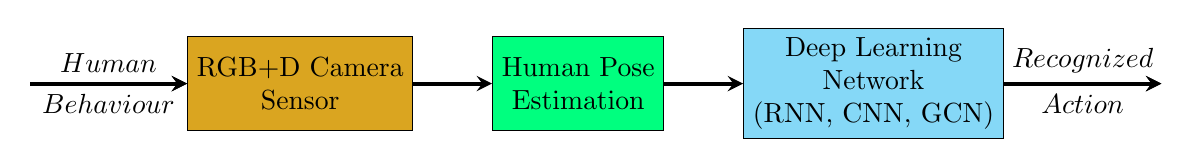
\begin{tikzpicture}
              \node[draw, align=center, fill=Goldenrod, minimum width=1cm, minimum height=1.2cm]  (cam) at (0,0) {RGB+D Camera\\ Sensor};
              \node[draw, align=center, fill=SpringGreen, minimum width=1cm, minimum height=1.2cm, right= 1cm of cam]  (pos) {Human Pose\\ Estimation};
              \node[draw, align=center, fill=ProcessBlue!50, minimum width=1cm, minimum height=1.2cm, right= 1cm of pos]  (nn) {Deep Learning\\ Network\\(RNN, CNN, GCN)};
              
              \draw[stealth-,  line width=0.05cm] (cam.west) -- ++ (-2,0) node[midway,above]{$Human$};
              \draw[stealth-,  line width=0.05cm] (cam.west) -- ++ (-2,0) node[midway,below]{$Behaviour$};
              
              \draw[-stealth,  line width=0.05cm] (cam.east) -- (pos.west);
              \draw[-stealth,  line width=0.05cm] (pos.east) -- (nn.west);
              
              \draw[-stealth,  line width=0.05cm] (nn.east) -- ++ (2,0) node[midway,above]{$Recognized$};
              \draw[-stealth,  line width=0.05cm] (nn.east) -- ++ (2,0) node[midway,below]{$Action$};
      \end{tikzpicture}
      }
\end{frame}

\begin{frame}{Lifelong Action Learning}
      \framesubtitle{}%
      
      \begin{itemize}
              \item Robotic systems fine-tune their knowledge with experience
              \item New actions are learnt while retaining the knowledge of the previous actions
              \item Concept of lifelong action learning was explored in the context of CRI
              \newline
              \item \textbf{Objectives}:
              \begin{itemize}
                  \item \small Develop an action learning model using incremental learning
                  \item \small Integrate model on QTRobot for the MigrAVE project
              \end{itemize}
      \end{itemize}
\end{frame}

\begin{frame}{Lifelong Action Learning}
      \framesubtitle{}%
      
      \begin{itemize}
              \item Efthymiou et al. work was first to look at IL with action recognition for CRI
              \item Edutainment system for scenarios such as classroom settings
      \end{itemize}
      
      \begin{figure}[h!]
              \centering
              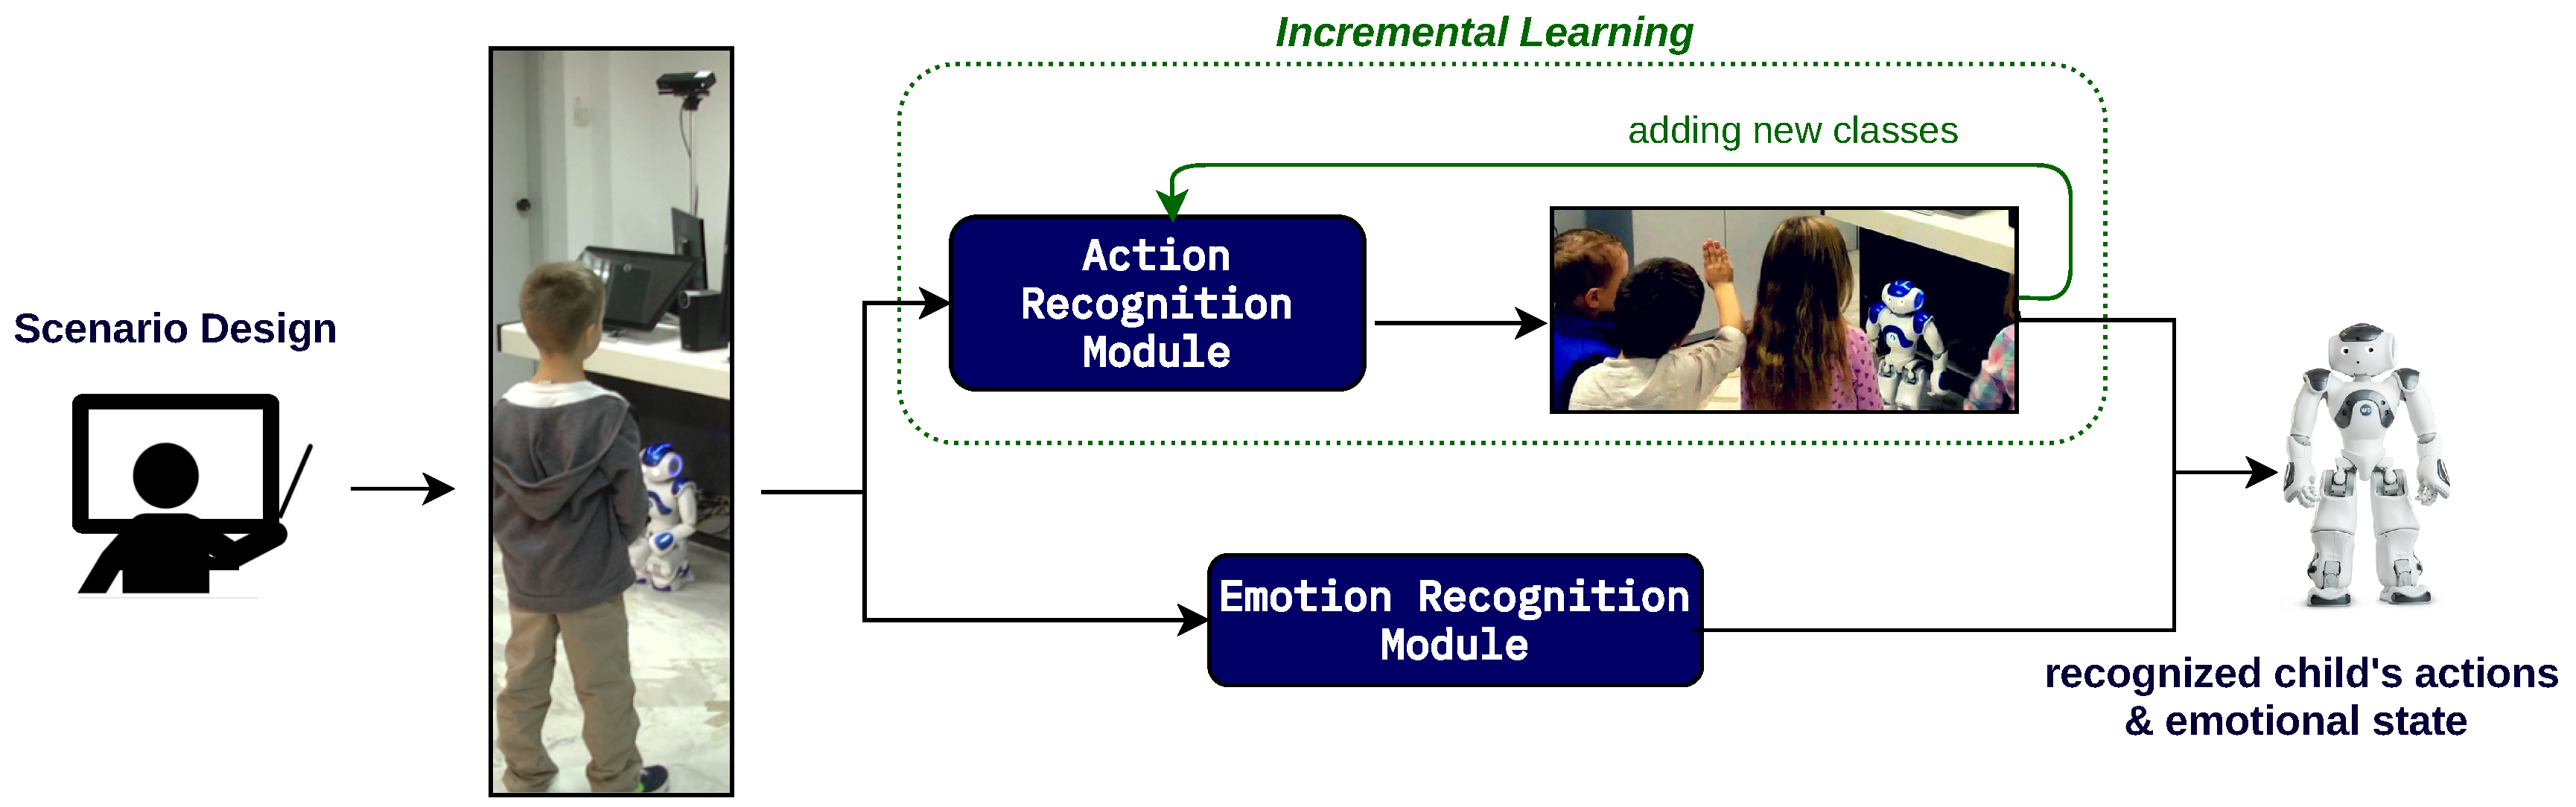
\includegraphics[width=0.9\textwidth]{images/IL_pipeline.png} 
              \caption{Incremental learning pipeline for action and emotion recognition\footnotemark}
      \end{figure} 
      \footnotetext{N. Efthymiou, P. P. Filntisis, G. Potamianos, and P. Maragos, “Visual Robotic Perception System with Incremental Learning for Child–Robot Interaction Scenarios,” Technologies, vol. 9, no. 86, November 2021.}
\end{frame}

\begin{frame}{Lifelong Action Learning}
      \framesubtitle{}%
      
      \begin{figure}[h!]
      \centering
      \begin{tikzpicture}
              \draw[red,thick,dashed] (0,0) ellipse (3cm and 1cm);
              \node(a){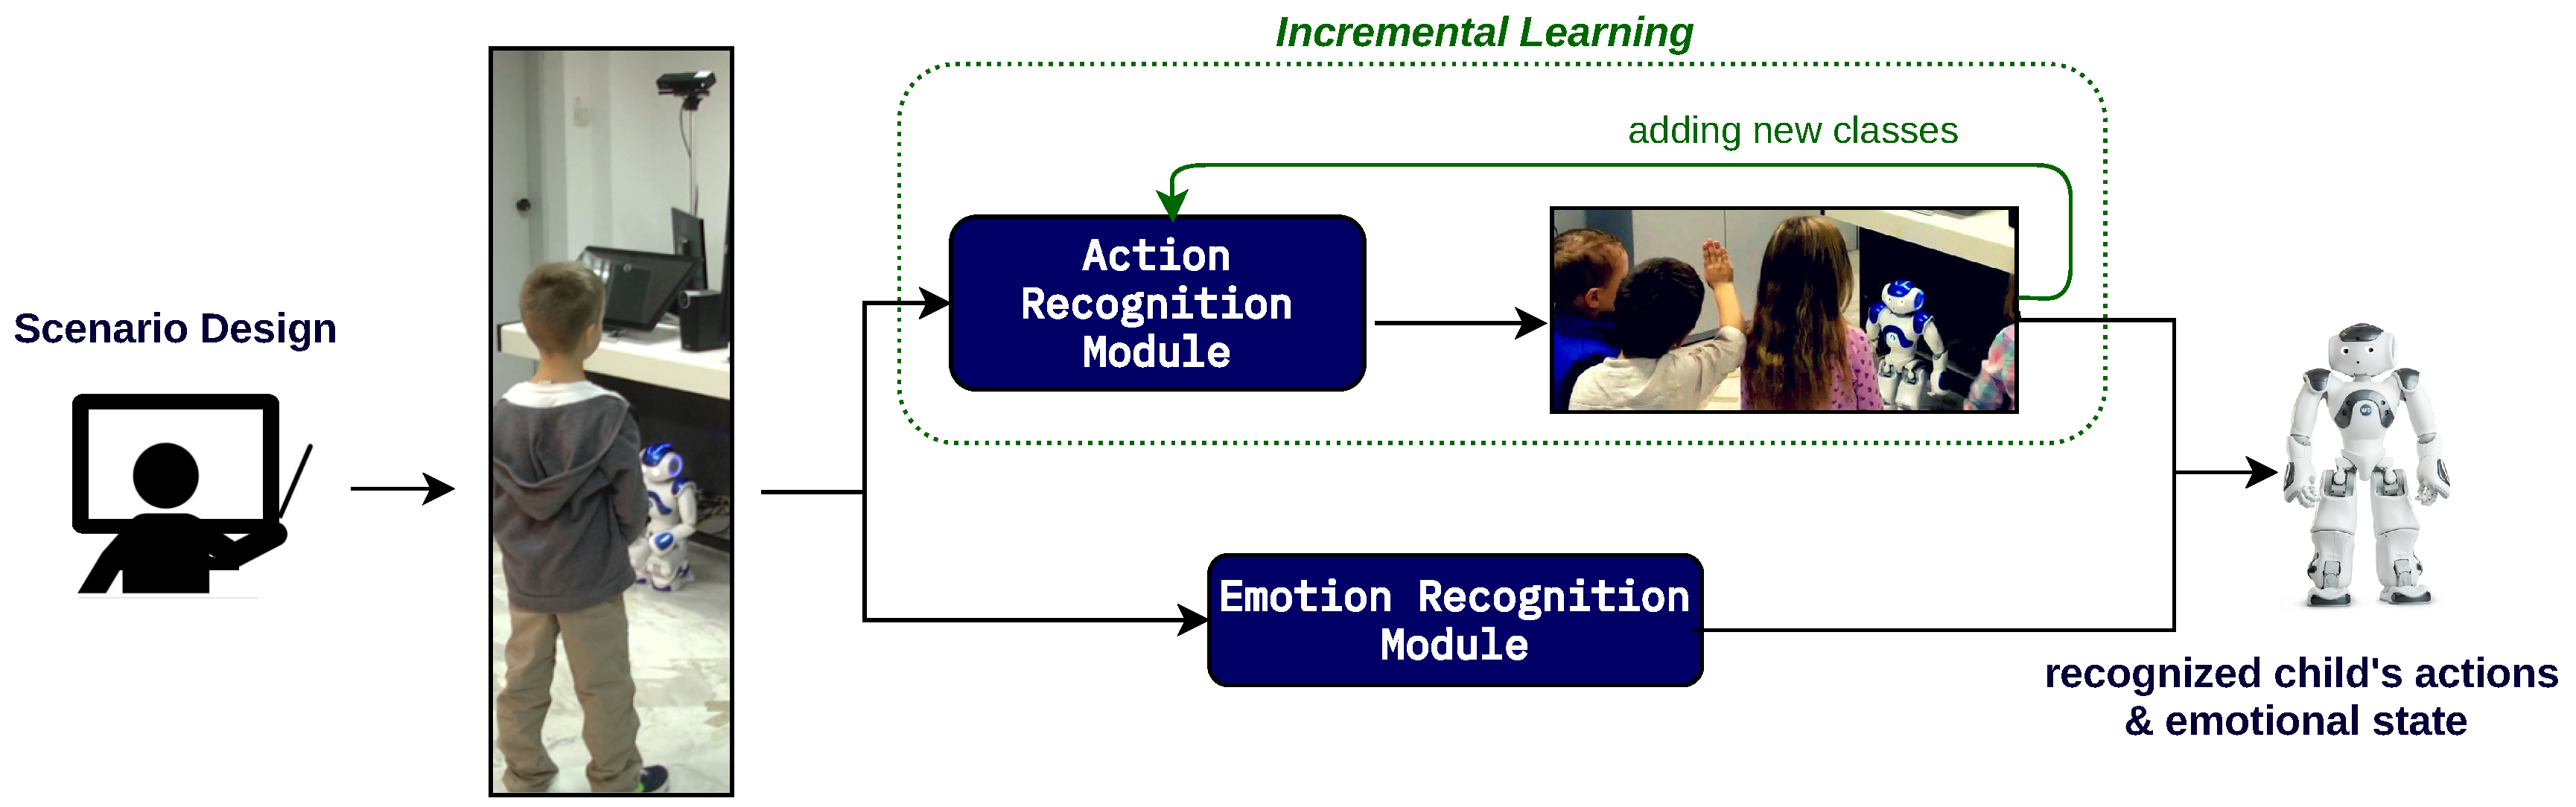
\includegraphics[width=0.9\textwidth]{images/IL_pipeline.png}};
              \node at (a.center) [draw, red, line width=3pt, ellipse, minimum width=200pt, minimum height=80pt, xshift=30pt, yshift=21pt]{};
      \end{tikzpicture}
      \caption{Incremental learning pipeline for action and emotion recognition\footnotemark[1]}
      \end{figure} 
      \footnotetext[1]{N. Efthymiou, P. P. Filntisis, G. Potamianos, and P. Maragos, “Visual Robotic Perception System with Incremental Learning for Child–Robot Interaction Scenarios,” Technologies, vol. 9, no. 86, November 2021.}
\end{frame}

\begin{frame}{Lifelong Action Learning}
      \framesubtitle{}%
      
      \begin{columns}
      \column{.5\textwidth}
      \begin{block}{Their Approach}
              \begin{itemize}
                  \item TSN Network
                  \item iCaRL Algorithm
                  \item RGB+D and Optical Flow data
                  \item BabyRobot Dataset
              \end{itemize}
      \end{block}
      
      \column{0.5\textwidth}
      \begin{block}{Our Approach}
              \begin{itemize}
                  \item CTR-GCN Network
                  \item BiC Algorithm
                  \item 3D Skeleton data
                  \item NTU RGB+D Dataset
              \end{itemize}
      \end{block}
      \end{columns}
\end{frame}

\begin{frame}{Our Approach}
      \framesubtitle{Methodology}%
      
      \begin{columns}
      \column{0.5\textwidth}
      \vspace{-0.75cm}
      \begin{enumerate}
              \item Performed a comparative analysis on skeleton-based action recognition networks
              \item Performed a comparative analysis on class-incremental learning algorithms
              \item Integrated the final model on QTRobot
      \end{enumerate}
      
      \column{0.5\textwidth}
      \begin{figure}[ht!]
            \centering
            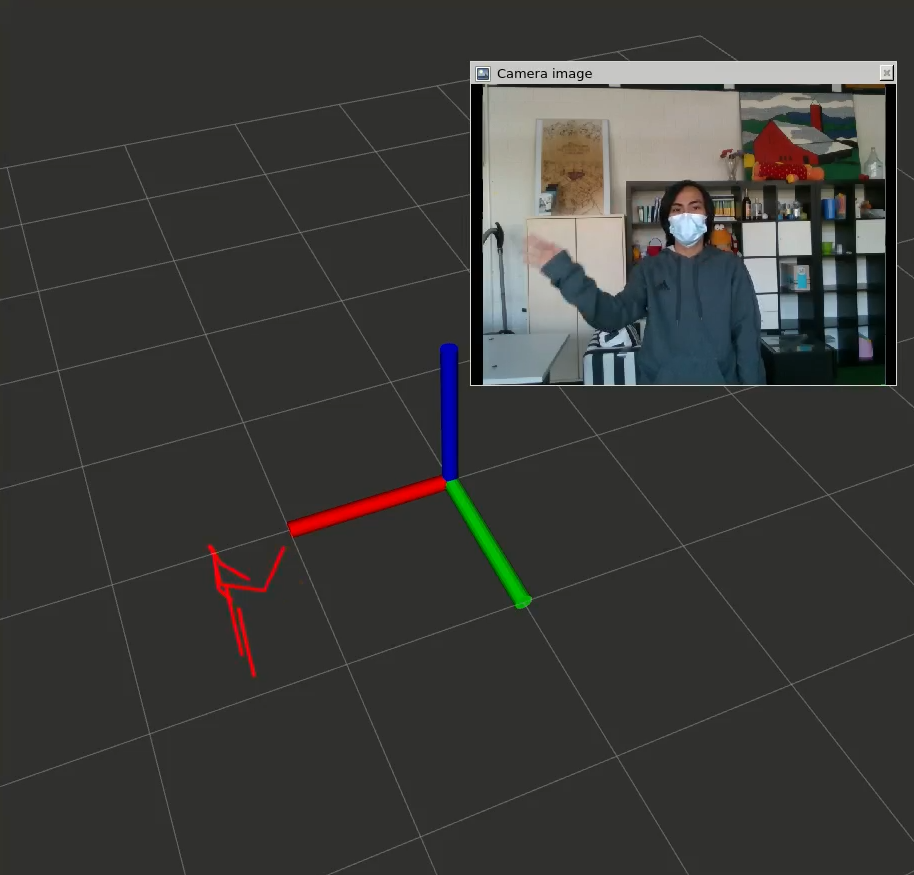
\includegraphics[width=0.7\textwidth]{images/waving_action_recognition.png}
            \caption{Hand waving action visualized in RVIZ}
      \end{figure}   
      \end{columns}
\end{frame}

\section{Comparative Analysis: Action Recognition}

\begin{frame}{NTU RGB+D Dataset}
      \framesubtitle{}%
      
      \vspace{-0.75cm}
      \begin{columns}
      \column{.45\textwidth}
      \begin{itemize}
            \item Features 120 everyday actions
            \item 40 subjects; 3 cameras; 2 demos
            \item 25 skeletal joints tracked
            \item Evaluation:
            \begin{itemize}
                  \item Cross-Subject Accuracy: train on 20 subjects; test on 20 subjects
                  \item Cross-View Accuracy: train using 2 views; test on 1 view
            \end{itemize}
      \end{itemize}
      
      \column{.55\textwidth}
      \begin{figure}[ht!]
            \centering
            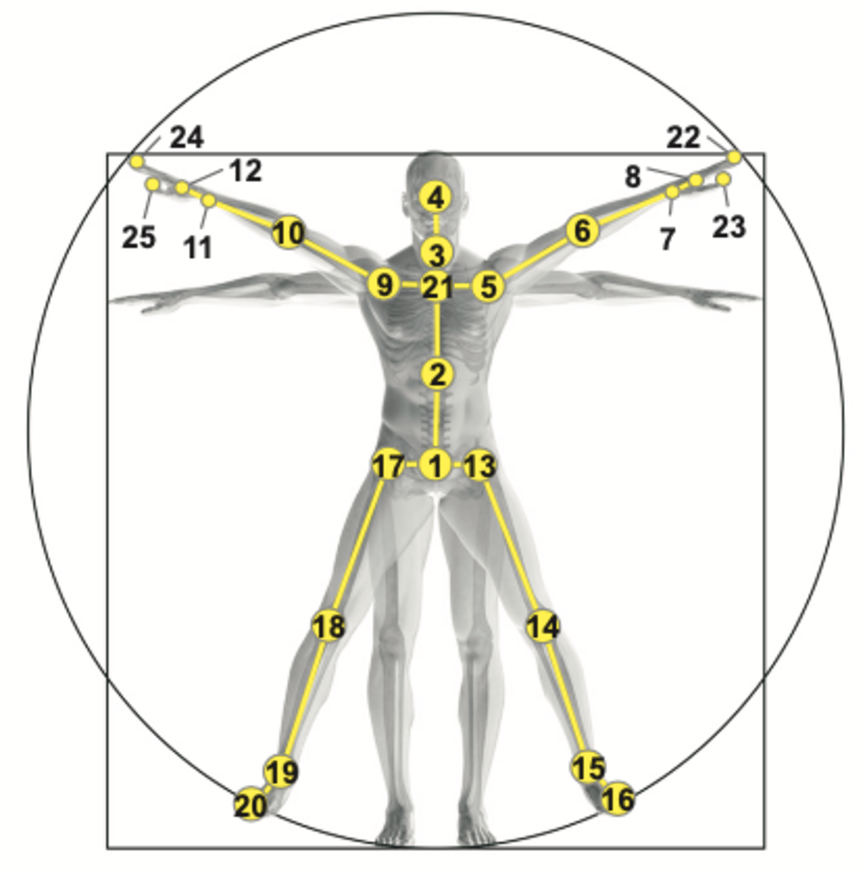
\includegraphics[width=0.7\textwidth]{images/joint_config.pdf}
            \caption{Joint configurations for NTU RGB-D dataset\footnotemark}
      \end{figure}      
      \end{columns}
      \footnotetext{A. Shahroudy, J. Liu, T.-T. Ng, and G. Wang, “NTU RGB+D: A Large Scale Dataset for 3D Human Activity Analysis,” in Proc. IEEE Conf. Computer Vision and Pattern Recognition (CVPR), 2016, pp. 1010–1019.}
\end{frame}

\begin{frame}{Action Recognition Analysis}
      \framesubtitle{}%
      
      \begin{itemize}
      \item Networks: CTR-GCN, MS-G3D, EfficientGCN, ViewAdaptive NN
      \item Modalities: Joint, Bone and Joint Motion
      \item \textbf{Metrics}: Cross-Subject \& Cross-View Accuracy \& Training Time
      \end{itemize}
      \vfill
      \begin{table}[ht!]
      \centering
      {\footnotesize
      \begin{tabular}{ |c|c|c|c| } 
              \hline
              Drink Water & Eat Meal & Brush Teeth & Drop \\ 
              \hline
              Pick Up & Throw & Sit Down & Stand Up \\ 
              \hline
              Clapping & Hand Waving & Kick Something & Hopping \\ 
              \hline
              Jump Up & Play with Phone & Point to Something & Rub Hands \\
              \hline
              Nod Head/Bow & Shake Head & Wipe Face & Cross Hands \\
              \hline
      \end{tabular}
      }
      \caption{Subset of action classes from the NTU RGB-D dataset}
      \end{table}
\end{frame}

\begin{frame}{Action Recognition Analysis Results}
      \framesubtitle{}%
      
      \begin{columns}
      \column{.6\textwidth}
      \begin{table}[h!]
      \centering
      {\footnotesize
      \begin{tabular}{ |C{0.32\textwidth}|C{0.32\textwidth}|C{0.25\textwidth}|C{0.2\textwidth}| } 
              \hline
              \rowcolor{gray!25}
              Network & Cross Subject & Cross View \\ 
              \hline
              CTR-GCN (Joint) & 92.63\% & 96.37\% \\ 
              \hline
              CTR-GCN (Bone) & \cellcolor{blue!25}92.78\% & 96.02\% \\ 
              \hline
              CTR-GCN (Motion) & 92.51\% & \cellcolor{blue!25}96.40\% \\ 
              \hline
              \hline
              MS-G3D (Joint) & \cellcolor{blue!25}91.27\% & \cellcolor{blue!25}96.85\% \\ 
              \hline
              MS-G3D (Bone) & 90.90\% & 95.44\% \\ 
              \hline
              \hline
              EfficientGCN-B4 (SG Layer) & 94.05\% & 97.47\% \\ 
              \hline
              EfficientGCN-B4 (EpSep Layer) & \cellcolor{blue!25}94.43\% & \cellcolor{blue!25}97.56\% \\ 
              \hline
              \hline
              VA-NN (CNN) & \cellcolor{blue!25}92.97\% & \cellcolor{blue!25}92.20\% \\
              \hline
              VA-NN (RNN) & - & - \\
              \hline
      \end{tabular}
      }
      \caption{Action recognition networks accuracy}
      \end{table}
      
      \column{.4\textwidth}
      \begin{table}[h!]
      \centering
      {\footnotesize
      \begin{tabular}{ |c|c| }
              \hline
              \rowcolor{gray!25}
              Network & Training Time \\
              \hline
              CTR-GCN & 4 hrs\\
              \hline
              MS-G3D & 8 hrs\\
              \hline
              EfficientGCN-B4 & 5 hrs\\
              \hline
              VA-NN & 0.5 hrs\\
              \hline
      \end{tabular}
      }
      \caption{Networks training time}     
      \end{table}
      \end{columns}
\end{frame}

\begin{frame}{Action Recognition Analysis Results}
      \framesubtitle{}%
      
      %\vspace{-0.25cm}
      \begin{table}[h!]
      \centering
      {\footnotesize
      \begin{tabular}{ | C{0.14\textwidth} | c | c || C{0.18\textwidth} | c | c | }
            \hline
            \rowcolor{gray!25}
            Action & CTR-GCN & MS-G3D & Action & CTR-GCN & MS-G3D \\
            \hline
            Drink Water & 82.48\% & \cellcolor{blue!25}83.94\% & Kick Something & \cellcolor{blue!25}97.83\% & 94.93\% \\
            \hline
            Eat Meal & \cellcolor{blue!25}78.91\% & 73.82\% & Hopping & \cellcolor{blue!25}98.91\% & 95.27\%  \\
            \hline
            Brush Teeth & 90.84\% & \cellcolor{blue!25}91.21\% & Jump Up & \cellcolor{blue!25}98.91\% & 98.55\% \\
            \hline
            Drop & 90.18\% & \cellcolor{blue!25}91.64\% & Play with Phone & 86.91\% & \cellcolor{blue!25}90.91\% \\
            \hline
            Pick Up & \cellcolor{blue!25}98.91\% & 94.55\% & Point to Something & \cellcolor{blue!25}92.39\% & 92.03\% \\
            \hline
            Throw & \cellcolor{blue!25}96.36\% & 90.91\% & Rub Hands & \cellcolor{blue!25}90.58\% & 89.49\% \\
            \hline
            Sit Down & \cellcolor{blue!25}98.90\% & 97.80\% & Nod Head/Bow & \cellcolor{blue!25}96.01\% & 95.65\% \\
            \hline
            Stand Up & 98.17\% & \cellcolor{blue!25}98.90\% & Shake Head & \cellcolor{blue!25}96.00\% & 95.64\% \\
            \hline
            Clapping & \cellcolor{blue!25}82.42\% & 72.89\% & Wipe Face & 92.39\% & \cellcolor{blue!25}94.20\% \\
            \hline
            Hand Waving & 94.16\% & \cellcolor{blue!25}94.89\% & Cross Hands & 93.84\% & \cellcolor{blue!25}94.57\% \\
            \hline
      \end{tabular}
      }
      \caption{Cross-Subject accuracy results per class for CTR-GCN and MS-G3D models}
      \end{table}
\end{frame}

\section{Comparative Analysis: Class-Incremental Learning}

\begin{frame}{Class-Incremental Learning}
      \framesubtitle{}%
      
      \begin{block}{Class-Incremental Learning Problem}
            \small An algorithm attempts to learn a given sequence of tasks, T:
            \begin{equation}
            \centering
            T = [ (C^1, D^1), (C^2, D^2), \ldots ,(C^n, D^n) ]
            \end{equation}
      \end{block}
      \vfill
      \begin{columns}
      \column{.55\textwidth}
      
      \begin{block}{Tasks}
            \small
            \begin{itemize}
            \item Set of actions to be learnt:
            \begin{equation}
            \centering
            D^t = \{ (x_1, y_1), \ldots, (x_{m^t}, y_{m^t}) \}
            \end{equation}
            \item Action set is distinct per task
            \begin{equation}
            \centering
            C^i \cap C^j = \oslash, \; if \; i \ne j
            \end{equation}
            \end{itemize}
      \end{block}
      
      \column{.45\textwidth}
      
      \begin{block}{Exemplars}
            \small
            \begin{itemize}
            \item Memory of training data from previous tasks
            \item Augments training data if $t > 1$
            \item Memory scenarios: fixed or growing
            \item Selection methods: random, herding, distance, entropy
            \end{itemize}
      \end{block}
      
      \end{columns}
\end{frame}

\begin{frame}{Class-Incremental Learning Metrics}
      \framesubtitle{}%
      
      \vspace{-0.35cm}
      \begin{columns}
      \column{.5\textwidth}
      \begin{block}{Task-Aware Accuracy}
            \small Calculated with the knowledge of the action classes learnt within each task.
      \end{block}
      \begin{block}{Task-Agnostic Accuracy}
            \small Calculated with the overall set of the action classes learnt.
      \end{block}
      
      \column{.5\textwidth}
      \begin{block}{Forgetting Percentage}
            \small Estimated percentage of data forgotten
            \begin{equation}
            \centering
            F_{i, t} = max(A[i, 0:t-1]) - A[i, t], \; i\leq t
            \end{equation}
            where i = evaluated task \& t = current task
      \end{block}
      
      \end{columns}
      \vfill
      \begin{figure}[ht!]
            \centering
            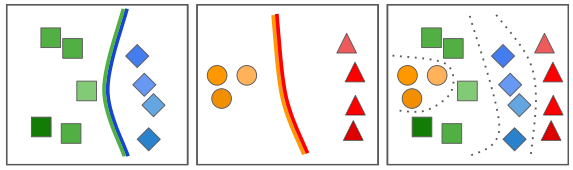
\includegraphics[width=0.45\textwidth]{images/IL_tasks}
            \caption{Incremental learning process of 4 classes split into 2 tasks\footnotemark}
      \end{figure} 
      \footnotetext{M. Masana et al., “Class-Incremental Learning: Survey and Performance Evaluation,” CoRR, vol. abs/2010.15277, October 2020.}
\end{frame}

\begin{frame}{Class-Incremental Learning Analysis}
      \framesubtitle{}%
      
      \vspace{-0.15cm}
      \begin{columns}
      \column{0.5\textwidth}
      \vspace{-0.75cm}
      \begin{itemize}
            \item IL Algorithms: LwF\footnotemark[4], iCaRL\footnotemark[5], LUCIR\footnotemark[6], BiC\footnotemark[7]
            \item Memory Size: 400 (Fixed) \& 20 per class (Growing)
            \item Selection Method: Random \& Herding
            \item \textbf{Metrics}: Task-Aware \& Task-Agnostic Accuracy
      \end{itemize}
      
      \column{0.65\textwidth}
      \begin{table}[ht!]
      \centering
      {\footnotesize
      \begin{tabular}{ | c | C{0.24\textwidth} || c | C{0.28\textwidth} | }
            \hline
            \rowcolor{gray!25}
            Task \# & Action & Task \# & Action \\
            \hline
            Task 1 & Wipe Face & Task 6 & Throw \\
                        & Eat Meal & & Point to Something \\ 
            \hline
            Task 2 & Cross Hands & Task 7 & Hand Waving \\ 
                        & Clapping & & Stand Up \\
            \hline
            Task 3 & Kick Something & Task 8 & Nod Head/Bow \\
                        & Shake Head & & Hopping \\
            \hline
            Task 4 & Sit Down & Task 9 & Drop \\
                        & Play with Phone & & Drink Water \\
            \hline
            Task 5 & Pick Up & Task 10 & Rub Hands \\
                        & Brush Teeth & & Jump Up \\
            \hline
      \end{tabular}
      }
      \caption{Task sequence for class-IL comparative analysis}
      \end{table}
      \end{columns}
      \footnotetext[4]{Z. Li and D. Hoiem, “Learning without Forgetting,” IEEE Trans. Pattern Analysis and Machine Intelligence, vol. 40, no. 12, pp. 2935–2947, Dec 2018.}
      \footnotetext[5]{S.-A. Rebuffi, A. Kolesnikov, G. Sperl, and C. H. Lampert, “iCaRL: Incremental Classifier and Representation Learning,” in Proc. IEEE Conf. Computer Vision and Pattern Recognition (CVPR), 2017, pp. 5533–5542.}
      \footnotetext[6]{S. Hou, X. Pan, C. C. Loy, Z. Wang, and D. Lin, “Learning a Unified Classifier Incrementally via Rebalancing,” in Proc. IEEE/CVF Conf. Computer Vision and Pattern Recognition (CVPR), 2019, pp. 831–839.}
      \footnotetext[7]{Y. Wu et al., “Large Scale Incremental Learning,” in Proc. IEEE/CVF Conf. Computer Vision and Pattern Recognition (CVPR), 2019, pp. 374–382.}
\end{frame}

\begin{frame}{Class-Incremental Learning Analysis}
      \framesubtitle{LwF, iCaRL, LUCIR Model Architecture}%
      
      \vspace{0.5cm}
      {\footnotesize
      \centering
      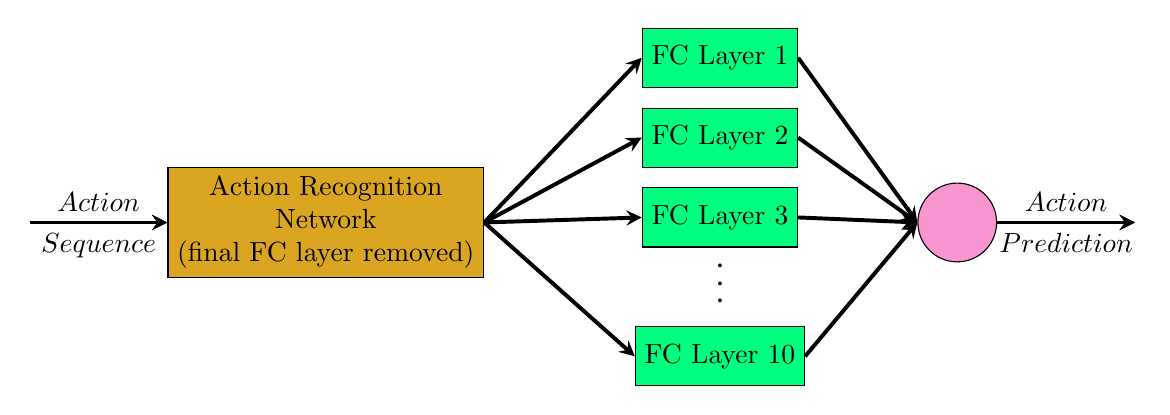
\begin{tikzpicture}
              \node[draw, align=center, fill=Goldenrod, minimum width=1cm, minimum height=1.2cm]  (net) at (0,0) {Action Recognition\\ Network\\ (final FC layer removed)};
              
              \node[draw, align=center, fill=SpringGreen, minimum width=1.5cm, minimum height=0.75cm, above right= 1cm and 2cm of net]  (head1) {FC Layer 1};
              \node[draw, align=center, fill=SpringGreen, minimum width=1.5cm, minimum height=0.75cm, below=0.25cm of head1]  (head2) {FC Layer 2};
              \node[draw, align=center, fill=SpringGreen, minimum width=1.5cm, minimum height=0.75cm, below=0.25cm of head2]  (head3) {FC Layer 3};
              \node[draw, align=center, fill=SpringGreen, minimum width=1.5cm, minimum height=0.75cm, below=1cm of head3]  (headt) {FC Layer 10};
              
              \node[draw, circle, minimum size=1cm, fill=Rhodamine!50, right= 5.5cm of net] (sum) {};
                            
              \path (head3) -- (headt) node [black, font=\Large, midway, sloped] {$\dots$};              
              \draw[stealth-,  line width=0.05cm] (net.west) -- ++ (-1.75,0) node[midway,above]{$Action$};
              \draw[stealth-,  line width=0.05cm] (net.west) -- ++ (-1.75,0) node[midway,below]{$Sequence$};
              
              \draw[-stealth,  line width=0.05cm] (net.east) -- (head1.west);
              \draw[-stealth,  line width=0.05cm] (net.east) -- (head2.west) node[midway,above]{};
              \draw[-stealth,  line width=0.05cm] (net.east) -- (head3.west) node[midway,above]{};
              \draw[-stealth,  line width=0.05cm] (net.east) -- (headt.west) node[midway,above]{};
                            
              \draw[-stealth,  line width=0.05cm] (head1.east) -- (sum.west) node[midway,above]{};
              \draw[-stealth,  line width=0.05cm] (head2.east) -- (sum.west) node[midway,above]{};
              \draw[-stealth,  line width=0.05cm] (head3.east) -- (sum.west) node[midway,above]{};
              \draw[-stealth,  line width=0.05cm] (headt.east) -- (sum.west) node[midway,above]{};
              
              \draw[-stealth,  line width=0.05cm] (sum.east) -- ++ (1.75,0) node[midway,above]{$Action$};
              \draw[-stealth,  line width=0.05cm] (sum.east) -- ++ (1.75,0) node[midway,below]{$Prediction$};
      \end{tikzpicture}
      }
\end{frame}

\begin{frame}{Class-Incremental Learning Analysis}
      \framesubtitle{BiC Model Architecture}%
      
      \vspace{0.5cm}
      {\footnotesize
      \centering
      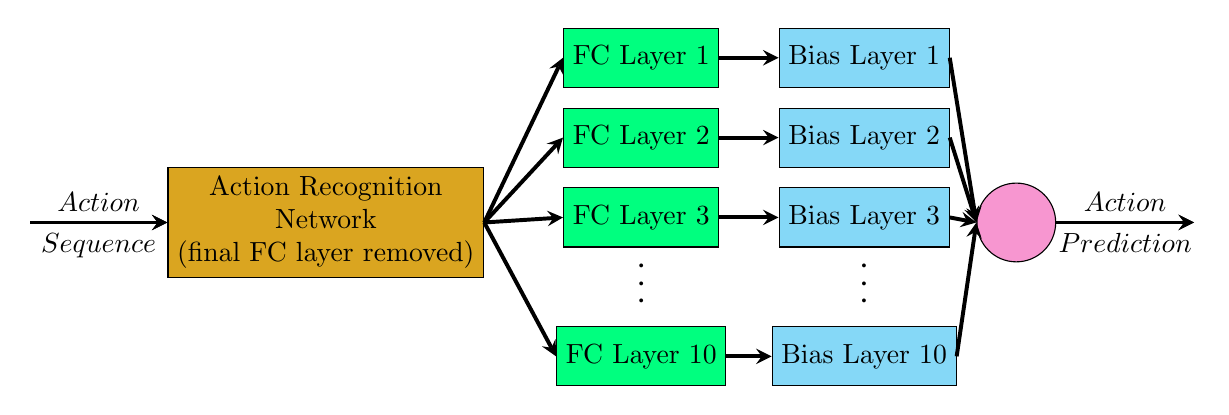
\begin{tikzpicture}
              \node[draw, align=center, fill=Goldenrod, minimum width=1cm, minimum height=1.2cm]  (net) at (0,0) {Action Recognition\\ Network\\ (final FC layer removed)};
              
              \node[draw, align=center, fill=SpringGreen, minimum width=1.5cm, minimum height=0.75cm, above right= 1cm and 1cm of net]  (head1) {FC Layer 1};
              \node[draw, align=center, fill=SpringGreen, minimum width=1.5cm, minimum height=0.75cm, below=0.25cm of head1]  (head2) {FC Layer 2};
              \node[draw, align=center, fill=SpringGreen, minimum width=1.5cm, minimum height=0.75cm, below=0.25cm of head2]  (head3) {FC Layer 3};
              \node[draw, align=center, fill=SpringGreen, minimum width=1.5cm, minimum height=0.75cm, below=1cm of head3]  (headt) {FC Layer 10};
              
              \node[draw, align=center, fill=ProcessBlue!50, minimum width=1.5cm, minimum height=0.75cm, right= 0.75cm of head1]  (bl1) {Bias Layer 1};
              \node[draw, align=center, fill=ProcessBlue!50, minimum width=1.5cm, minimum height=0.75cm, below=0.25cm of bl1]  (bl2) {Bias Layer 2};
              \node[draw, align=center, fill=ProcessBlue!50, minimum width=1.5cm, minimum height=0.75cm, below=0.25cm of bl2]  (bl3) {Bias Layer 3};
              \node[draw, align=center, fill=ProcessBlue!50, minimum width=1.5cm, minimum height=0.75cm, below=1cm of bl3]  (blt) {Bias Layer 10};
              
              \node[draw, circle, minimum size=1cm, fill=Rhodamine!50, right= 6.25cm of net] (sum) {};
                            
              \path (head3) -- (headt) node [black, font=\Large, midway, sloped] {$\dots$};
              \path (bl3) -- (blt) node [black, font=\Large, midway, sloped] {$\dots$};
              
              \draw[stealth-,  line width=0.05cm] (net.west) -- ++ (-1.75,0) node[midway,above]{$Action$};
              \draw[stealth-,  line width=0.05cm] (net.west) -- ++ (-1.75,0) node[midway,below]{$Sequence$};
              
              \draw[-stealth,  line width=0.05cm] (net.east) -- (head1.west);
              \draw[-stealth,  line width=0.05cm] (net.east) -- (head2.west) node[midway,above]{};
              \draw[-stealth,  line width=0.05cm] (net.east) -- (head3.west) node[midway,above]{};
              \draw[-stealth,  line width=0.05cm] (net.east) -- (headt.west) node[midway,above]{};
                            
              \draw[-stealth,  line width=0.05cm] (head1.east) -- (bl1.west) node[midway,above]{};
              \draw[-stealth,  line width=0.05cm] (head2.east) -- (bl2.west) node[midway,above]{};
              \draw[-stealth,  line width=0.05cm] (head3.east) -- (bl3.west) node[midway,above]{};
              \draw[-stealth,  line width=0.05cm] (headt.east) -- (blt.west) node[midway,above]{};
              
              \draw[-stealth,  line width=0.05cm] (bl1.east) -- (sum.west) node[midway,above]{};
              \draw[-stealth,  line width=0.05cm] (bl2.east) -- (sum.west) node[midway,above]{};
              \draw[-stealth,  line width=0.05cm] (bl3.east) -- (sum.west) node[midway,above]{};
              \draw[-stealth,  line width=0.05cm] (blt.east) -- (sum.west) node[midway,above]{};
              
              \draw[-stealth,  line width=0.05cm] (sum.east) -- ++ (1.75,0) node[midway,above]{$Action$};
              \draw[-stealth,  line width=0.05cm] (sum.east) -- ++ (1.75,0) node[midway,below]{$Prediction$};
      \end{tikzpicture}
      }
\end{frame}

\begin{frame}{Class-Incremental Learning Analysis Results}
      \framesubtitle{Training Time}%
      
      %\vspace{-0.65cm}
      \begin{table}[ht!]
      \centering
      {\footnotesize
      \begin{tabular}{ | >{\columncolor{gray!25}}c | >{\columncolor{gray!25}}C{1.2cm} | C{1.37cm} | C{1.55cm} | C{1.3cm} || C{1.37cm} | C{1.55cm} | C{1.3cm} | }
            \hline
            \rowcolor{gray!25}
            & & \multicolumn{3}{c ||}{CTR-GCN} & \multicolumn{3}{c |}{MS-G3D} \\
            \hline
            \rowcolor{gray!25}
            Algorithm & Memory Config & Total Time (hrs) & Time per Task (min) & Time Incr per Task & Total Time (hrs) & Time per Task (min) & Time Incr per Task \\
            \hline
            iCaRL & Fixed & 6.3 & 18.9 \& 39.2 & - & 11.2 & 30.2 \& 68.7 & - \\
            \cline{2-8}
            & Growing & 5.6 & - & 2.8\% & 11.0 & - & 2.6\% \\
            \hline
            LWF & Fixed & 6.6 & 19.9 \& 41.8 & - & 11.3 & 30.6 \& 69.6 & - \\
            \cline{2-8}
            & Growing & 5.8 & - & 2.8\% & 10.1 & - & 2.9\% \\
            \hline
            BIC & Fixed & 7.0 & \cellcolor{blue!25}19.6 \& 44.1 & - & 11.5 & 30.2 \& 68.2 & - \\
            \cline{2-8}
            & Growing & 6.2 & - & \cellcolor{blue!25}3.3\% & 10.4 & - & 2.6\% \\
            \hline
            LUCIR & Fixed & 6.4 & 19.6 \& 39.6 & - & 11.4 & 33.0 \& 71.4 & - \\
            \cline{2-8}
            & Growing & 5.8 & - & 2.9\% & 10.1 & - & 2.9\% \\
            \hline
      \end{tabular}
      }
      \caption{Incremental learning model training time}
      \end{table}
\end{frame}

\begin{frame}{Class-Incremental Learning Analysis Results}
      \framesubtitle{Task-Aware Accuracy}%
      
      \begin{table}[ht!]
      \centering
      {\footnotesize
      \begin{tabular}{ | >{\columncolor{gray!25}}c | >{\columncolor{gray!25}}C{1.2cm} | C{1.55cm} | C{1.55cm} || C{1.55cm} | C{1.55cm} | }
            \hline
            \rowcolor{gray!25}
            & & \multicolumn{2}{c ||}{Herding} & \multicolumn{2}{c |}{Random} \\
            \hline
            \rowcolor{gray!25}
            Algorithm & Memory Config & CTR-GCN & MS-G3D  & CTR-GCN & MS-G3D \\
            \hline
            iCaRL & Fixed & 94.9\% & 97.2\% & 95.3\% & 98.1\% \\
            \cline{2-6}
            & Growing & 91.1\% & 95.9\% & 91.2\% & 96.6\% \\
            \hline
            LWF & Fixed & 98.4\% & 97.8\% & 98.2\% & 97.5\% \\
            \cline{2-6}
            & Growing & 97.6\% & 96.1\% & 97.1\% & 96.1\% \\
            \hline
            LUCIR & Fixed & 95.5\% & 97.5\% & 97.3\% & 97.5\% \\
            \cline{2-6}
            & Growing & 96.3\% & 94.8\% & 95.5\% & 96.5\% \\
            \hline
            BiC & Fixed & \cellcolor{blue!25}98.2\% & 98.1\% & 97.9\% & 96.9\% \\
            \cline{2-6}
            & Growing & \cellcolor{blue!25}97.3\% & 96.9\% & 97.5\% & 96.6\% \\
            \hline
      \end{tabular}
      }
      \caption{Average task-aware accuracy }
      \end{table}
\end{frame}

\begin{frame}{Class-Incremental Learning Analysis Results}
      \framesubtitle{Task-Agnostic Accuracy}%
      
      \begin{table}[ht!]
      \centering
      {\footnotesize
      \begin{tabular}{ | >{\columncolor{gray!25}}c | >{\columncolor{gray!25}}C{1.2cm} | C{1.55cm} | C{1.55cm} || C{1.55cm} | C{1.55cm} | }
            \hline
            \rowcolor{gray!25}
            & & \multicolumn{2}{c ||}{Herding} & \multicolumn{2}{c |}{Random} \\
            \hline
            \rowcolor{gray!25}
            Algorithm & Memory Config & CTR-GCN & MS-G3D  & CTR-GCN & MS-G3D \\
            \hline
            iCaRL & Fixed & 52.1\% & 72.5\% & 50.9\% & 72.1\% \\
            \cline{2-6}
            & Growing & 54.2\% & 67.8\% & 51.3\% & 66.9\% \\
            \hline
            LWF & Fixed & 73.8\% & 67.8\%  & 75.4\% & 67.5\% \\
            \cline{2-6}
            & Growing & 69.9\% & 61.5\% & 69.4\% & 63.5\% \\
            \hline
            LUCIR & Fixed & 66.2\% & 64.7\% & 68.4\% & 64.4\% \\
            \cline{2-6}
            & Growing & 65.5\% & 43.6\% & 62.4\% & 59.9\% \\
            \hline
            BiC & Fixed & \cellcolor{blue!25}79.1\% & 70.1\% & 74.8\% & 67.1\% \\
            \cline{2-6}
            & Growing & \cellcolor{blue!25}74.2\% & 61.1\% & 72.8\% & 61.6\% \\
            \hline
      \end{tabular}
      }
      \caption{Average task-agnostic accuracy}
      \end{table}
\end{frame}

\begin{frame}{Class-Incremental Learning Analysis}
      \framesubtitle{How would the model perform if we grouped similar actions?}%
      
      \vspace{0.5cm}
      \begin{columns}
      \column{0.45\textwidth}
      \vspace{-0.75cm}
      \begin{itemize}
            \item Task-Aware Accuracy: 
            \begin{itemize}
                  \item \small Fixed: 98.2\% $\Longrightarrow$ 94.6\%
                  \item \small Growing: 97.3\% $\Longrightarrow$ 93.4\%
            \end{itemize}
            \item Task-Agnostic Accuracy: 
            \begin{itemize}
                  \item \small Fixed: 79.1\% $\Longrightarrow$ 77.6\%
                  \item \small Growing: 74.2\% $\Longrightarrow$ 72.7\%
            \end{itemize}
      \end{itemize}
      
      \column{0.65\textwidth}
      \begin{table}[ht!]
      \centering
      {\footnotesize
      \begin{tabular}{ | c | C{0.24\textwidth} || c | C{0.28\textwidth} | }
            \hline
            \rowcolor{gray!25}
            Task \# & Action & Task \# & Action \\
            \hline
            Task 1 & Brush Teeth & Task 5 & Clapping \\
            & Wipe Face & & Rub Hands \\ 
            \cline{1-2}
            Task 2 & Drink Water & & Cross Hands \\ 
            \cline{3-4}
            & Eat Meal & Task 6 & Hand Waving \\
            \cline{1-2}
            Task 3 & Drop & & Point to Something \\
            \cline{3-4}
            & Pick Up & Task 7 & Kick Something \\
            & Throw & & Hopping\\
            \cline{1-2}
            Task 4 & Sit Down & & Jump Up \\
            \cline{3-4}
            & Stand Up & Task 8 & Play with Phone \\
            \hline
            & & Task 9 & Nod Head/Bow \\
            & & & Shake Head \\
            \hline
      \end{tabular}
      }
      \caption{Task sequence with variable task size and sorting similar actions}
      \end{table}
      \end{columns}
\end{frame}

\begin{frame}{Class-Incremental Learning Analysis}
      \framesubtitle{Model Robustness}%
      
      \vspace{0.25cm}
      \begin{columns}
      \column{0.5\textwidth}
      \begin{itemize}
            \item Task-Aware Accuracy: 
            \begin{itemize}
                  \item \small Fixed: 94.6\% $\Longrightarrow$ 94.1\% \& 96.7\%
                  \item \small Growing: 93.4\% $\Longrightarrow$ 95.1\% \& 95.6\%
            \end{itemize}
      \end{itemize}
      \column{0.5\textwidth}
      \begin{itemize}
            \item Task-Agnostic Accuracy: 
            \begin{itemize}
                  \item \small Fixed: 77.6\% $\Longrightarrow$ 76.3\% \& 78.5\%
                  \item \small Growing: 72.7\% $\Longrightarrow$ 74.5\% \& 70.6\%
            \end{itemize}
      \end{itemize}
      \end{columns}
      \vspace{0.6cm}
      {\footnotesize
      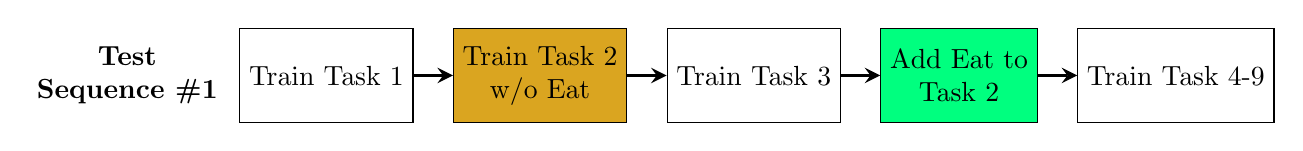
\begin{tikzpicture}
            \node[align=center, fill=white, minimum width=1cm, minimum height=1.2cm]  (t0) at (0,0) {\textbf{Test}\\ \textbf{Sequence \#1}};
            \node[draw, align=center, fill=white, minimum width=1cm, minimum height=1.2cm, right=0.15cm of t0] (t1) {Train Task 1};
            \node[draw, align=center, fill=Goldenrod, minimum width=1cm, minimum height=1.2cm, right=0.5cm of t1]  (t2) {Train Task 2\\ w/o Eat};
            \node[draw, align=center, fill=white, minimum width=1cm, minimum height=1.2cm, right=0.5cm of t2]  (t3) {Train Task 3};
            \node[draw, align=center, fill=SpringGreen, minimum width=1cm, minimum height=1.2cm, right=0.5cm of t3]  (t4) {Add Eat to\\ Task 2};
            \node[draw, align=center, fill=white, minimum width=1cm, minimum height=1.2cm, right=0.5cm of t4]  (t5) {Train Task 4-9};
            
            \draw[-stealth,  line width=0.05cm] (t1.east) -- (t2.west);
            \draw[-stealth,  line width=0.05cm] (t2.east) -- (t3.west);
            \draw[-stealth,  line width=0.05cm] (t3.east) -- (t4.west);
            \draw[-stealth,  line width=0.05cm] (t4.east) -- (t5.west);
      \end{tikzpicture}
      }
      \vspace{0.75cm}

      {\footnotesize
      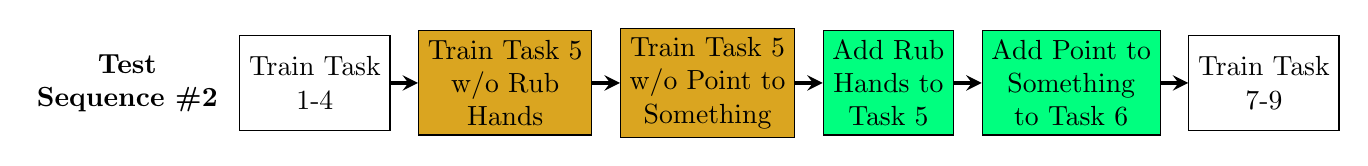
\begin{tikzpicture}
            \node[align=center, fill=white, minimum width=1cm, minimum height=1.2cm]  (t0) at (0,0) {\textbf{Test}\\ \textbf{Sequence \#2}};
            \node[draw, align=center, fill=white, minimum width=1cm, minimum height=1.2cm, right=0.15cm of t0] (t1) {Train Task\\ 1-4};
            \node[draw, align=center, fill=Goldenrod, minimum width=1cm, minimum height=1.2cm, right=0.35cm of t1]  (t2) {Train Task 5\\ w/o Rub\\ Hands};
            \node[draw, align=center, fill=Goldenrod, minimum width=1cm, minimum height=1.2cm, right=0.35cm of t2]  (t3) {Train Task 5\\ w/o Point to\\ Something};
            \node[draw, align=center, fill=SpringGreen, minimum width=1cm, minimum height=1.2cm, right=0.35cm of t3]  (t4) {Add Rub\\ Hands to\\ Task 5};
            \node[draw, align=center, fill=SpringGreen, minimum width=1cm, minimum height=1.2cm, right=0.35cm of t4]  (t5) {Add Point to\\ Something\\ to Task 6};
            \node[draw, align=center, fill=white, minimum width=1cm, minimum height=1.2cm, right=0.35cm of t5]  (t6) {Train Task\\ 7-9};
            
            \draw[-stealth,  line width=0.05cm] (t1.east) -- (t2.west);
            \draw[-stealth,  line width=0.05cm] (t2.east) -- (t3.west);
            \draw[-stealth,  line width=0.05cm] (t3.east) -- (t4.west);
            \draw[-stealth,  line width=0.05cm] (t4.east) -- (t5.west);
            \draw[-stealth,  line width=0.05cm] (t5.east) -- (t6.west);
      \end{tikzpicture}
      }
\end{frame}

\begin{frame}{Class-Incremental Learning Analysis}
      \framesubtitle{Memory Size}%
      
      \begin{table}[ht!]
      \centering
      {\footnotesize
      \begin{tabular}{ | C{0.75cm} | C{0.75cm} | C{0.75cm} | C{0.75cm} | C{0.75cm} | C{0.75cm} || C{0.75cm} | C{0.75cm} | C{0.75cm} | C{0.75cm} | C{0.75cm} | }
            \hline
            \multicolumn{6}{| c ||}{\cellcolor{gray!25}Growing} & \multicolumn{5}{c |}{\cellcolor{gray!25}Fixed} \\
            \hline
            2 & 5 & 10 & 20 & 50 & 100 & 40 & 100 & 200 & 400 & 1000 \\
            \hline
            78.3\% & 94.3\% & 97.2\% & \cellcolor{blue!25}97.3\% & 98.5\% & 98.7\% & 94.5\% & 96.7\% & 97.6\% & 98.2\% & 98.5\% \\
            \hline
      \end{tabular}
      }
      \caption{Average task-aware accuracy for varying memory size}
      \end{table}
      
      \vspace{-0.25cm}
      \begin{table}[ht!]
      \centering
      {\footnotesize
      \begin{tabular}{ | C{0.75cm} | C{0.75cm} | C{0.75cm} | C{0.75cm} | C{0.75cm} | C{0.75cm} || C{0.75cm} | C{0.75cm} | C{0.75cm} | C{0.75cm} | C{0.75cm} | }
            \hline
            \multicolumn{6}{| c ||}{\cellcolor{gray!25}Growing} & \multicolumn{5}{c |}{\cellcolor{gray!25}Fixed} \\
            \hline
            2 & 5 & 10 & 20 & 50 & 100 & 40 & 100 & 200 & 400 & 1000 \\
            \hline
            11.3\% & 45.7\% & 63.8\% & \cellcolor{blue!25}74.2\% & 79.8\% & 84.1\% & 35.8\% & 65.2\% & 70.3\% & 79.1\% & 80.0\% \\
            \hline
      \end{tabular}
      }
      \caption{Average task-agnostic accuracy for varying memory size}
      \end{table}

      \begin{itemize}
            \item Fixed memory is not feasable in real-life application (18\%-20\% time increase)
            \item Recording 50 or 100 demos of an action too onerous for performance benefit
            \item \textbf{Final Model}: CTR-GCN network, BiC algorithm, Growing memory (20/class), Herding selection
      \end{itemize}     
\end{frame}

\section{Assistive Robot Integration}

\begin{frame}{QTRobot Platform}
      \framesubtitle{}%
      
      \begin{columns}
      \column{0.5\textwidth}
      \vspace{-0.75cm}
      \begin{itemize}
            \item Teaching assistant for educators working with children
            \item Equipped with a RealSense 3D camera
            \item Skeletal tracking using Nuitrack SDK (19 joints tracked vs 25 joints in NTU)
      \end{itemize}

      \column{0.5\textwidth}
      \begin{figure}[ht!]
            \centering
            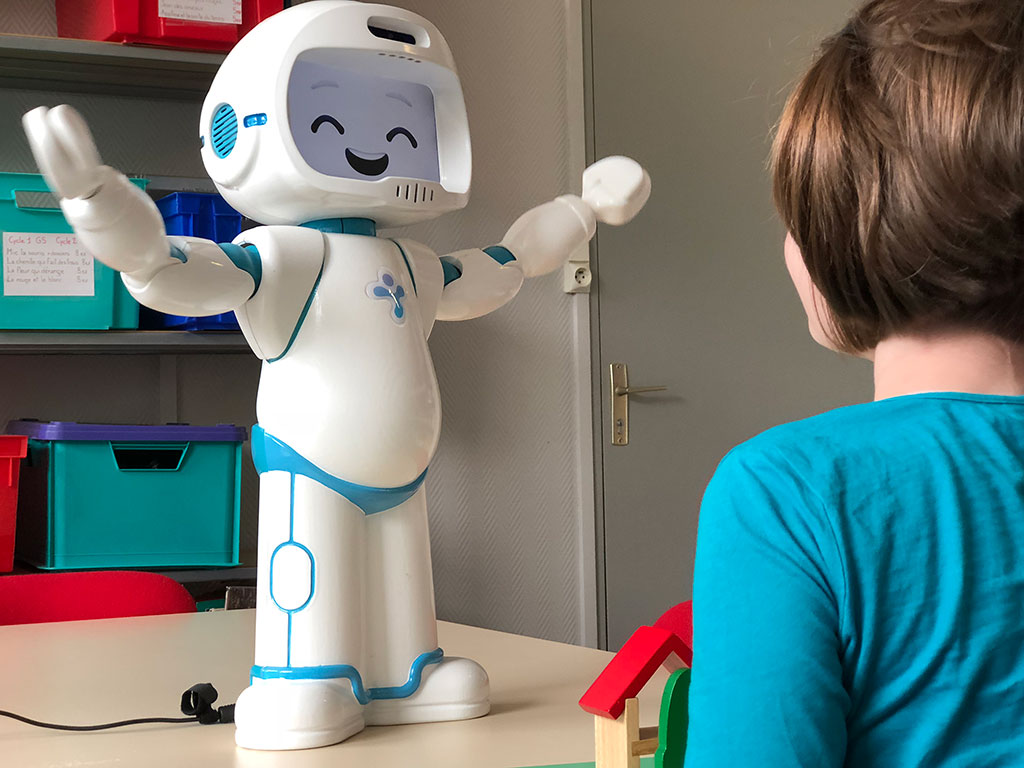
\includegraphics[width=0.8\textwidth]{images/qtrobot_with_child.jpeg}
            \caption{QTRobot interacting with a child\footnotemark[8]}
      \end{figure}
      \end{columns}
      \footnotetext[8]{Image taken from: https://robots.ieee.org/robots/qtrobot/} 
\end{frame}

\begin{frame}{Model Integration}
      \framesubtitle{}%
      
      \vspace{-0.25cm}
      \begin{columns}
      \column{0.55\textwidth}
       \begin{itemize}
            \item Task-Aware Accuracy: {\small 97.3\% $\Longrightarrow$ 97.4\%}
            \item Task-Agnostic Accuracy: {\small 74.2\% $\Longrightarrow$ 71.9\%}
      \end{itemize}
      \vspace{-0.4cm}
      \begin{figure}[h!]
      \centering
      \begin{tikzpicture}
              \node (a) {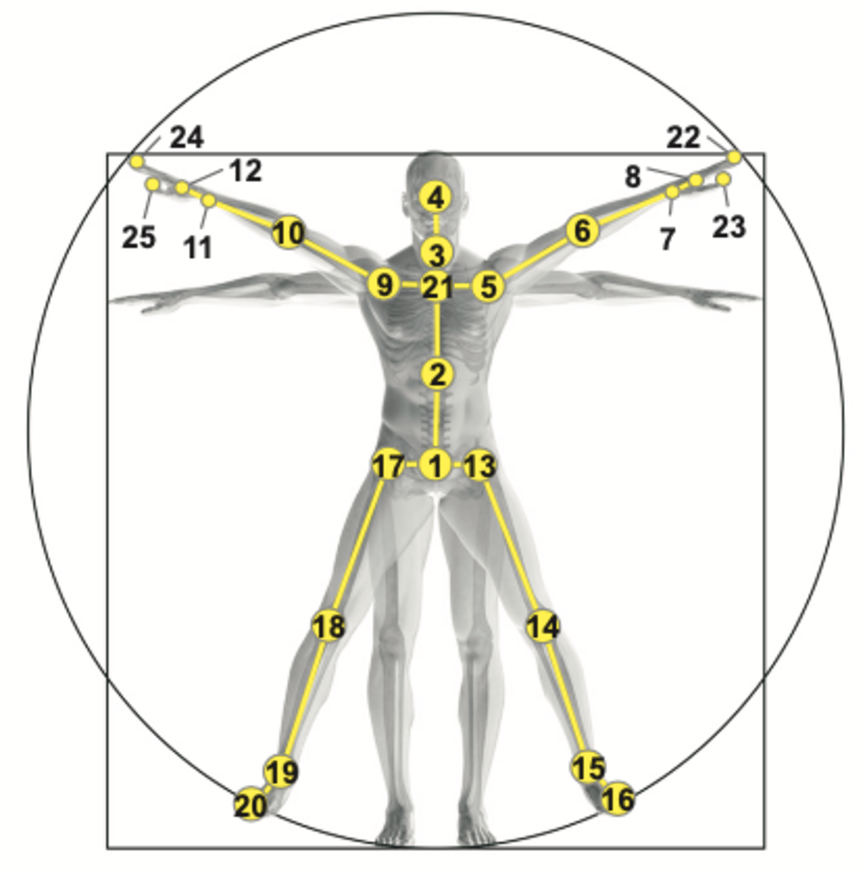
\includegraphics[trim=10 10 5 5,clip, width=0.475\textwidth]{images/joint_config.pdf}};
              
              \draw[red] (-1.1,1.29) circle (0.1cm and 0.1cm); %24
              \draw[red] (1.07,1.29) circle (0.1cm and 0.1cm); %22
              \draw[red] (-1.31,0.85) circle (0.1cm and 0.1cm); %25
              \draw[red] (1.28,0.89) circle (0.1cm and 0.1cm); %23
              \draw[red] (-0.82,-1.65) circle (0.1cm and 0.1cm); %20
              \draw[red] (0.79,-1.62) circle (0.1cm and 0.1cm); %16
      \end{tikzpicture}
      \caption{Joint configurations for NTU RGB-D dataset\footnotemark[9]}
      \end{figure} 
      
      \column{0.5\textwidth}
      \begin{figure}[ht!]
            \centering
            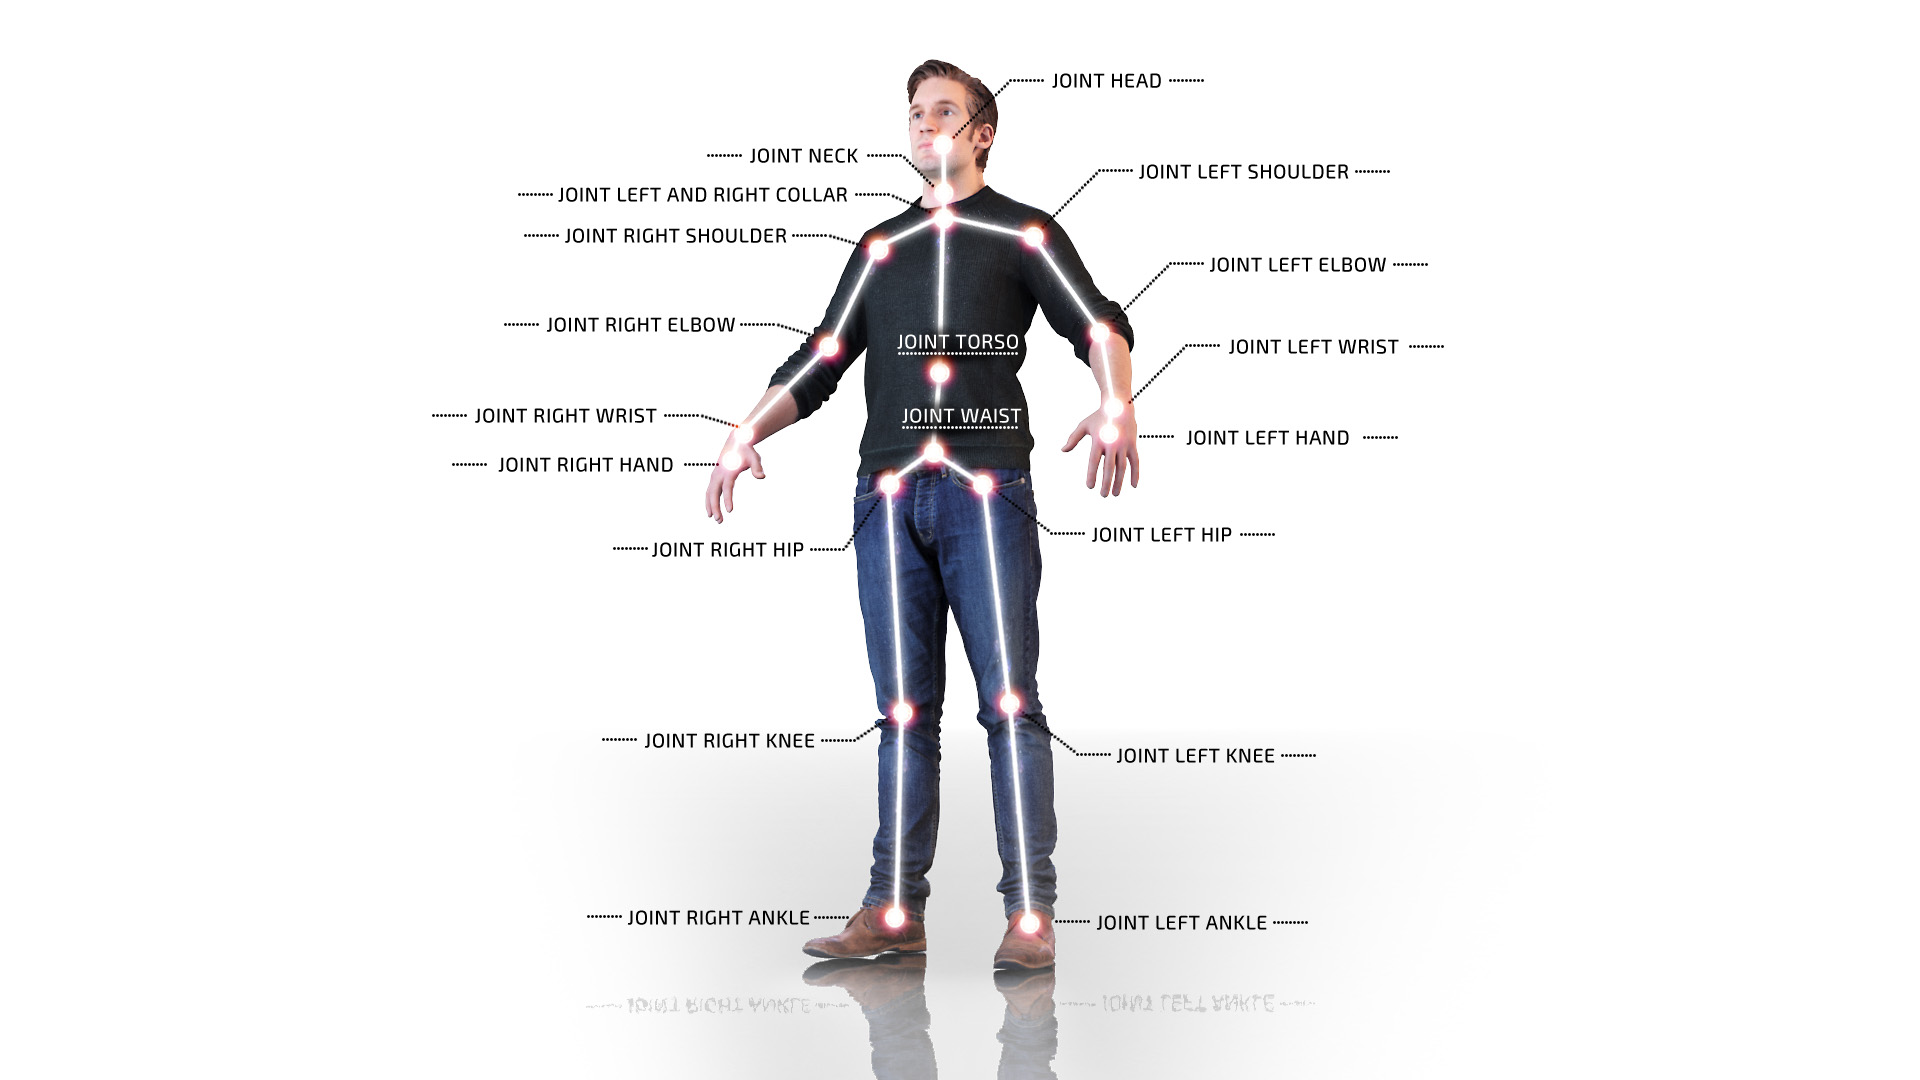
\includegraphics[trim=425 100 425 60,clip, width=0.8\textwidth]{images/nt_joints_config.jpeg}
            \caption{Joint configuration in the Nuitrack SDK\footnotemark[10]}
      \end{figure}
      \end{columns}
      \footnotetext[9]{A. Shahroudy, J. Liu, T.-T. Ng, and G. Wang, “NTU RGB+D: A Large Scale Dataset for 3D Human Activity Analysis,” in Proc. IEEE Conf. Computer Vision and Pattern Recognition (CVPR), 2016, pp. 1010–1019.}
      \footnotetext[10]{Image taken from: https://github.com/3DiVi/nuitrack-sdk/tree/master/doc}
\end{frame}

\begin{frame}{CAL Server}
      \framesubtitle{}%
      
      \begin{columns}
      \column{0.375\textwidth}
      \vspace{-0.75cm}
      \begin{itemize}
            \item ROS module w/ FTSM arch
            \item Two main subcomponents:
            \begin{itemize}
                  \item \small ActionClassifier
                  \item \small ActionLearner
            \end{itemize}
            \item Skeleton processor active after initialization
            \item Actions are classified with a 50 frame moving window
            \item Actions are learnt by capturing 25 demos
      \end{itemize}

      \column{0.85\textwidth}
      \vspace{-1.25cm}
      \begin{figure}[ht!]
            \centering
            %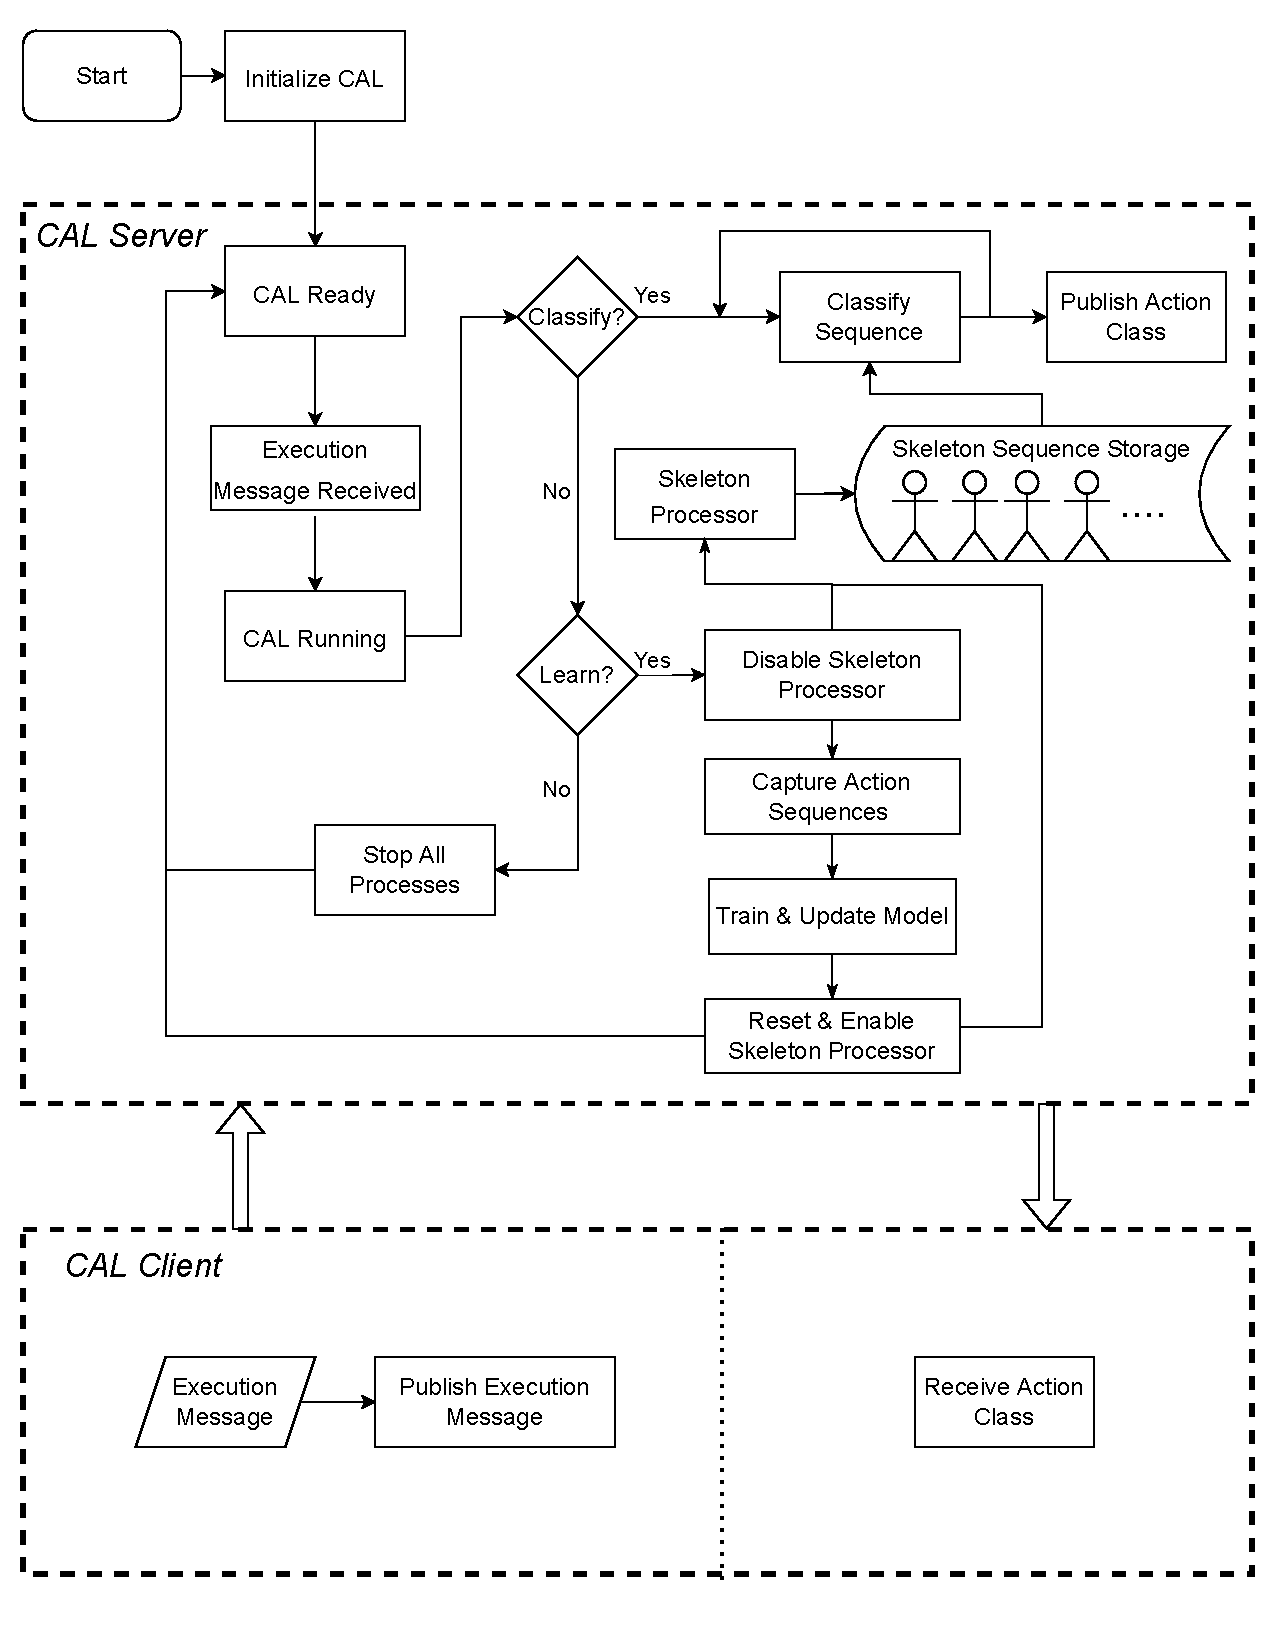
\includegraphics[trim=10 262 10 10,clip, width=0.7\textwidth]{images/CAL_workflow.pdf}
            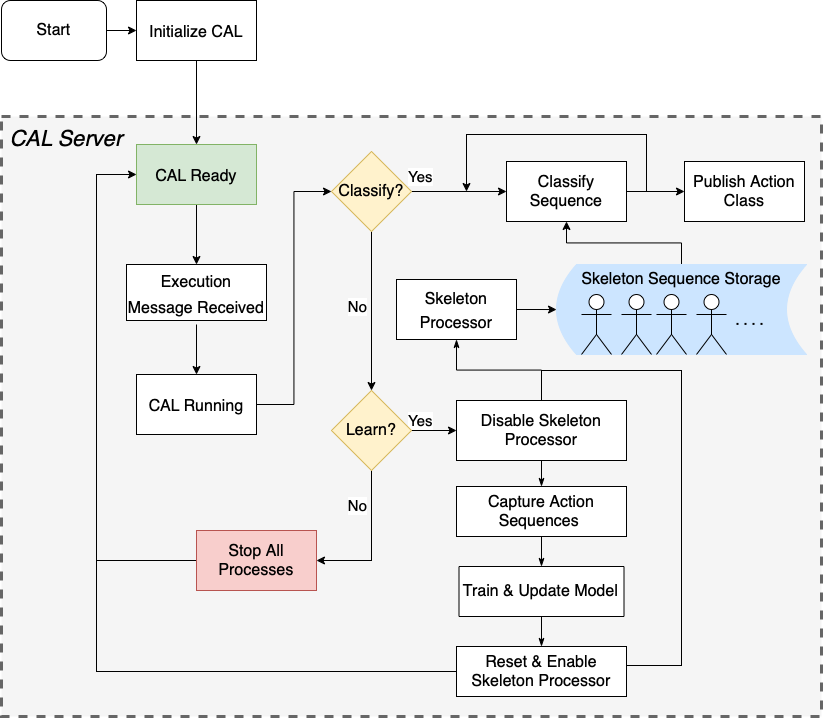
\includegraphics[width=0.7\textwidth]{images/CAL_workflow.png}
            \caption{Workflow of the Continual Action Learning Server}
      \end{figure}
      \end{columns}      
\end{frame}

\begin{frame}{Future Work}
      \framesubtitle{}%
      
      \begin{itemize}
            \item Investigating optimal number of frames for effective recognition
            \item Generation of synthetic trajectories to reduce learning efforts
            \item Investigating the effectiveness of model in HRI study 
      \end{itemize}
\end{frame}

\section{Human-Robot Interaction Study}

\begin{frame}{HRI Study}
      \framesubtitle{Experimental Design}%
      
      %\vspace{-0.25cm}
      \begin{columns}
      \column{0.7\textwidth}
      \vspace{-0.25cm}
      \begin{itemize}
            %\item \textbf{Goal}: Evaluate the robot's ability to recognize and learn new actions from user demo
            \item Three-part experiment:
            {\small
            \begin{enumerate}
                  \item The robot attempted to recognize users performing actions using the trained model
                  \item The robot recorded users perform 4 actions (2 new and 2 old) 25 times
                  \item The robot attempted to recognize users performing actions using the 3 experimental models
            \end{enumerate}
            }
            \vspace{0.5cm}
            \item \textbf{Performed Actions}: {\small Play with Phone, Hopping, Rub Hands, Hand Waving, Shake Head, Drink Water}
            \item \textbf{Learnt Actions}: {\small Talking on Phone, Cutting Food, Hand Waving, Hopping}
      \end{itemize}
      
      \column{0.35\textwidth}
      \begin{figure}[ht!]
            \centering
            \includegraphics[width=0.75\textwidth]{images/hri-study-setup}
            \caption{Robot and evaluator setup for HRI study}
      \end{figure} 
      \end{columns}
\end{frame}

\begin{frame}{Demo}
      \framesubtitle{Action Recognition}%
      
      \centering
      \movie[externalviewer]{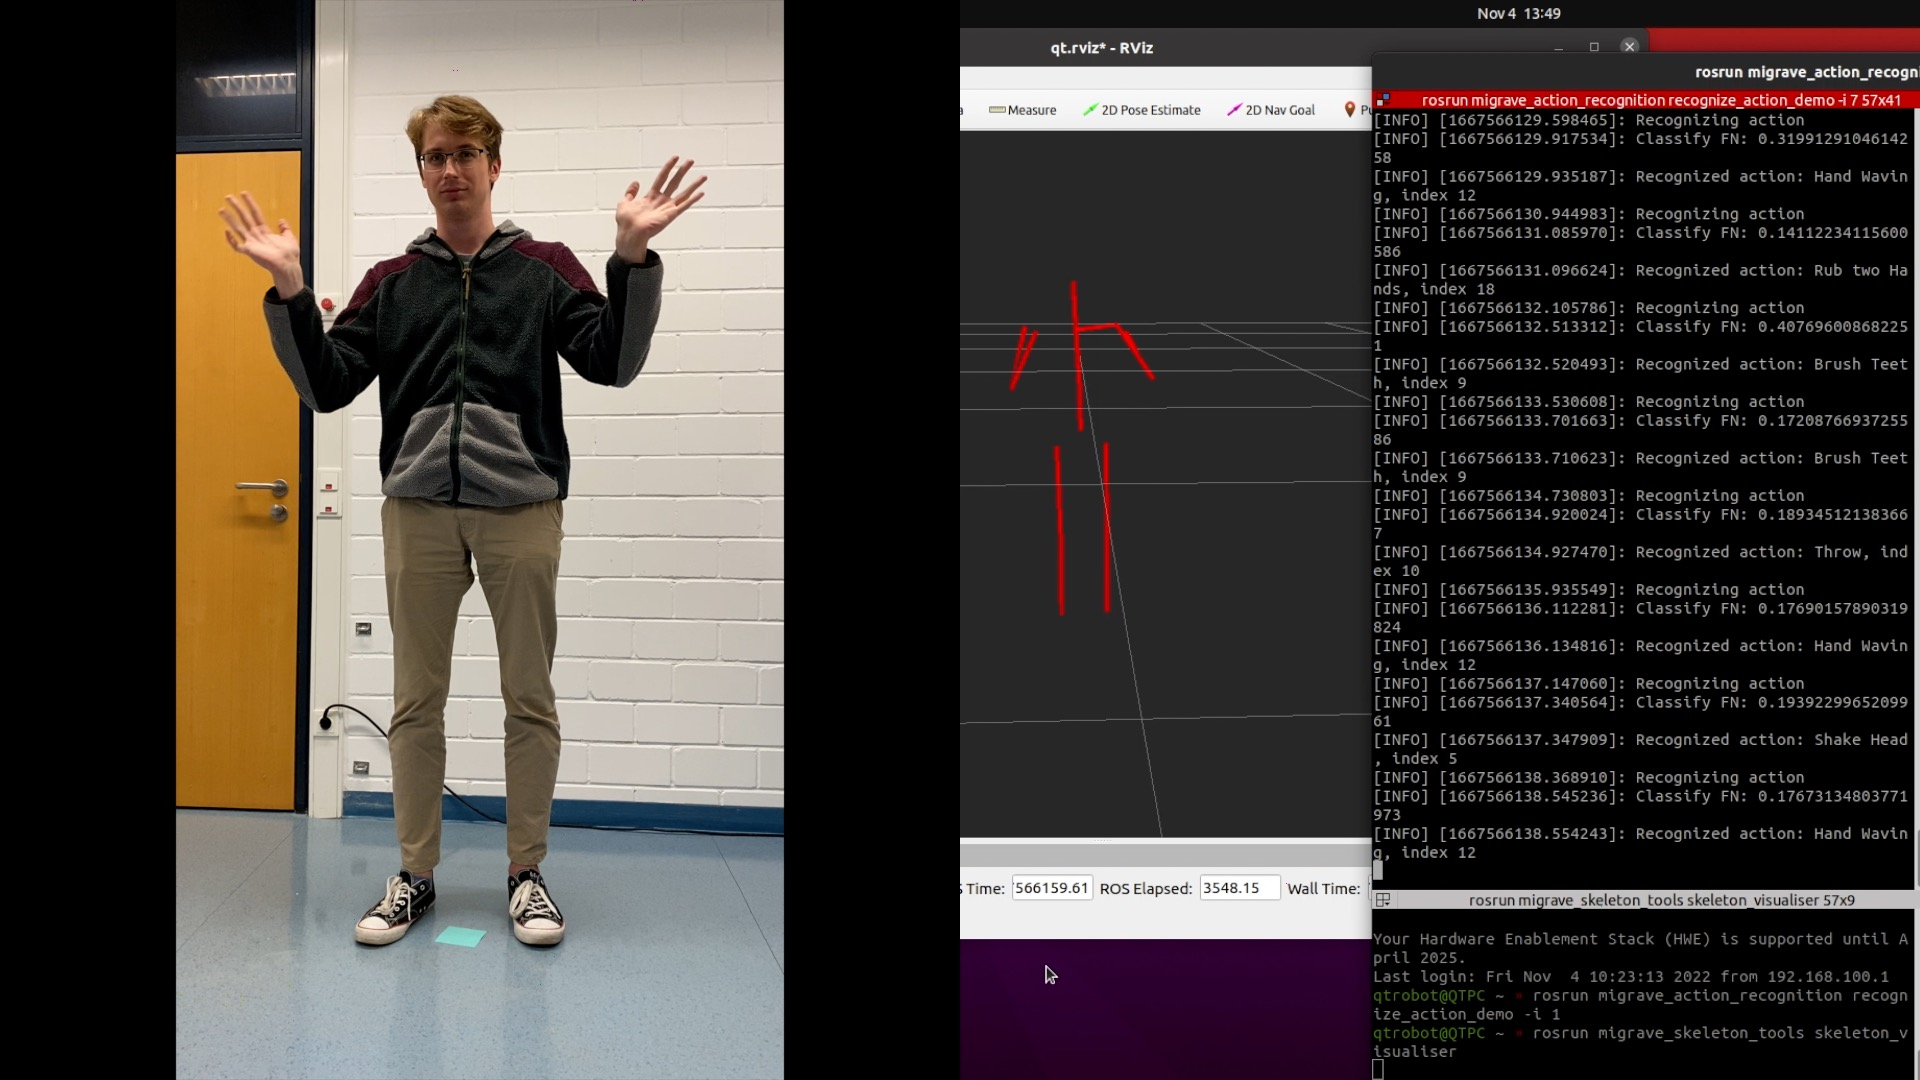
\includegraphics[width=0.75\textwidth, keepaspectratio]{images/LAL-ActionRecognition-poster.jpg}}{images/LAL-ActionRecognition.mp4}
\end{frame}

\begin{frame}{Demo}
      \framesubtitle{Action Learning}%
      
      \centering
      \movie[externalviewer]{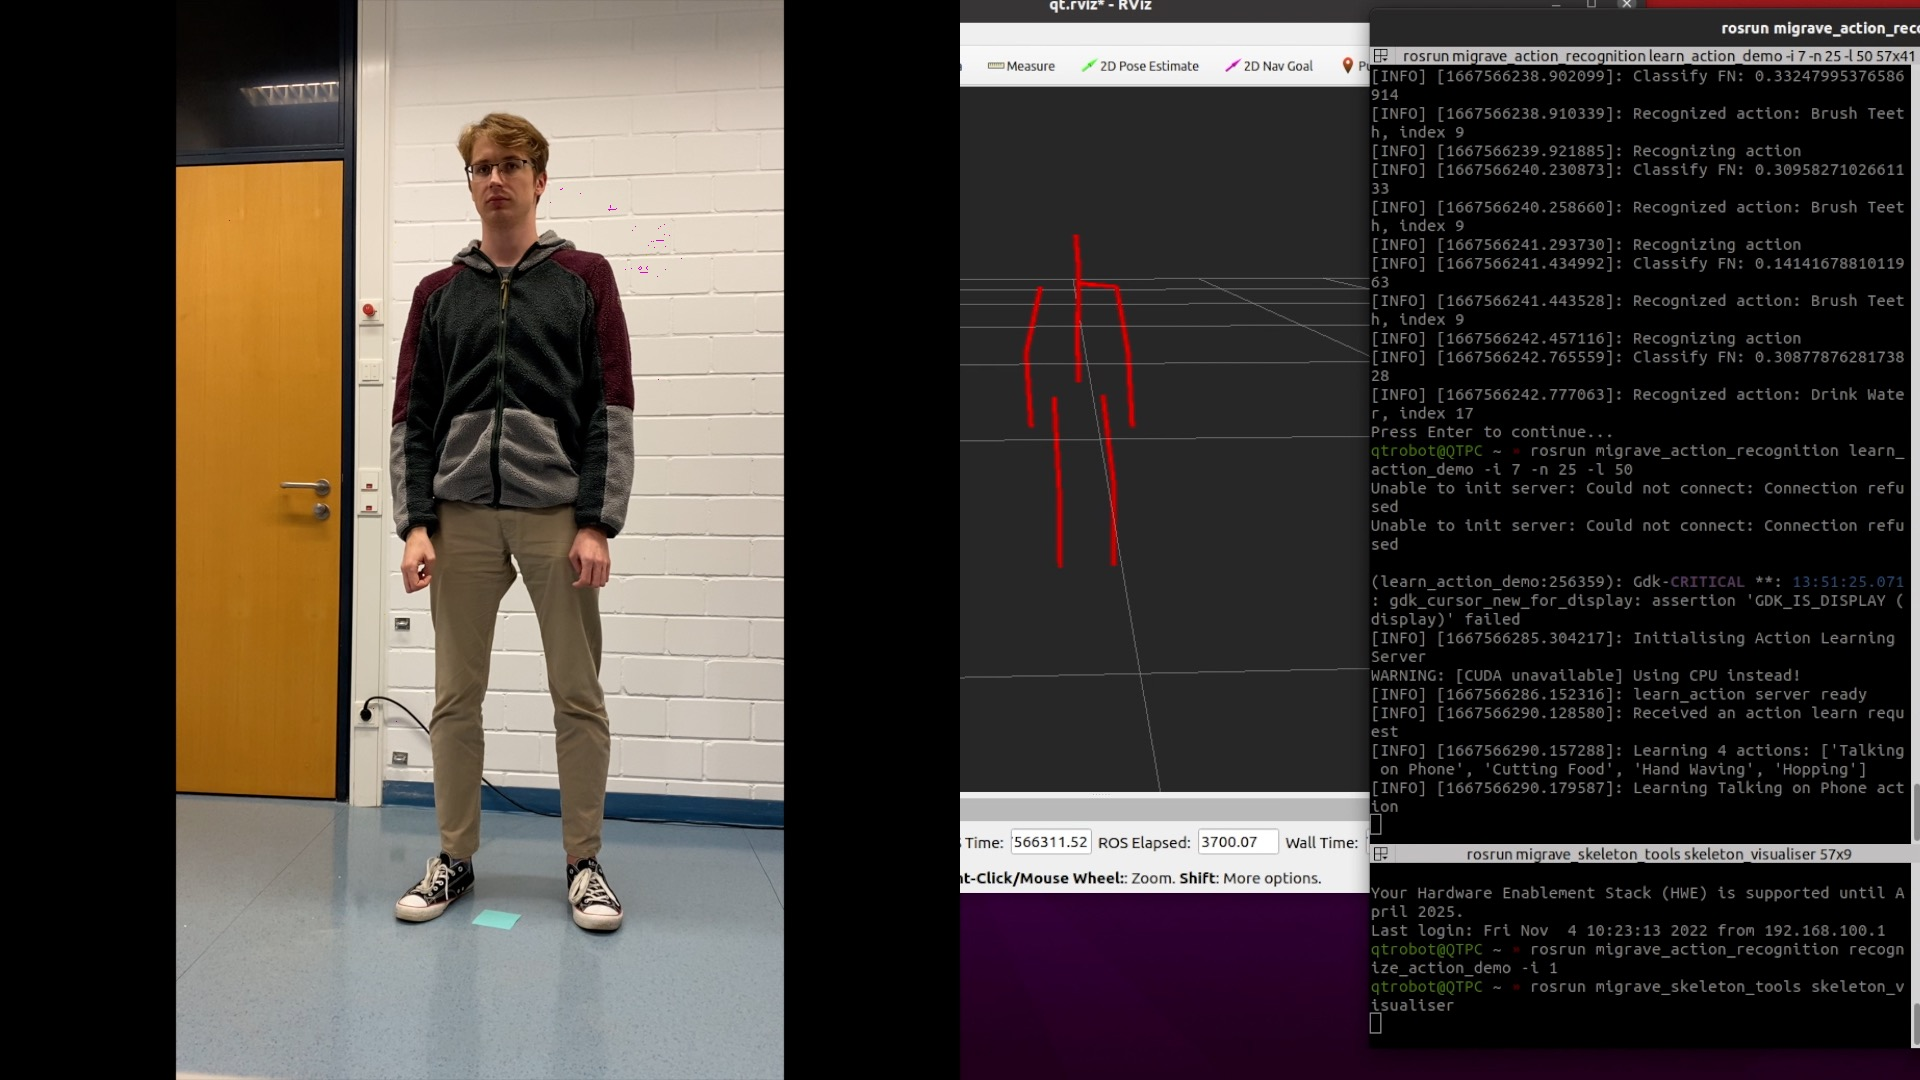
\includegraphics[width=0.75\textwidth, keepaspectratio]{images/LAL-ActionLearning-poster.jpg}}{images/LAL-ActionLearning.mp4}
\end{frame}

\begin{frame}{HRI Study}
      \framesubtitle{Results}%
      
      \vspace{-1cm}
      \begin{columns}
      \column{0.475\textwidth}
      \vspace{1cm}
      \begin{itemize}
            \item 15 users participated 
            \item Four models evaluated
            {\small
            \begin{enumerate}
                  \item Original trained model
                  \item Inclusion of 2 new actions as a new task
                  \item Improvement of old actions with new data
                  \item Modifying old task with new action
            \end{enumerate}
            }
      \end{itemize}
      \vspace{-0.25cm}
      \begin{table}[ht!]
      \centering
      {\footnotesize
      \begin{tabular}{ | c | c | }
            \hline
            \rowcolor{gray!25}
            Model & Accuracy \\
            \hline
            Original & 62.4\% \\
            \hline
            Exp. \#1 & 45.9\% \\
            \hline
            Exp. \#2 & 57.0\% \\
            \hline
            Exp. \#3 & 36.0\% \\
            \hline
      \end{tabular}
      }
      \caption{Accuracy per model}
      \end{table}
      
      \column{0.65\textwidth}
      \begin{figure}[ht!]
            \centering
            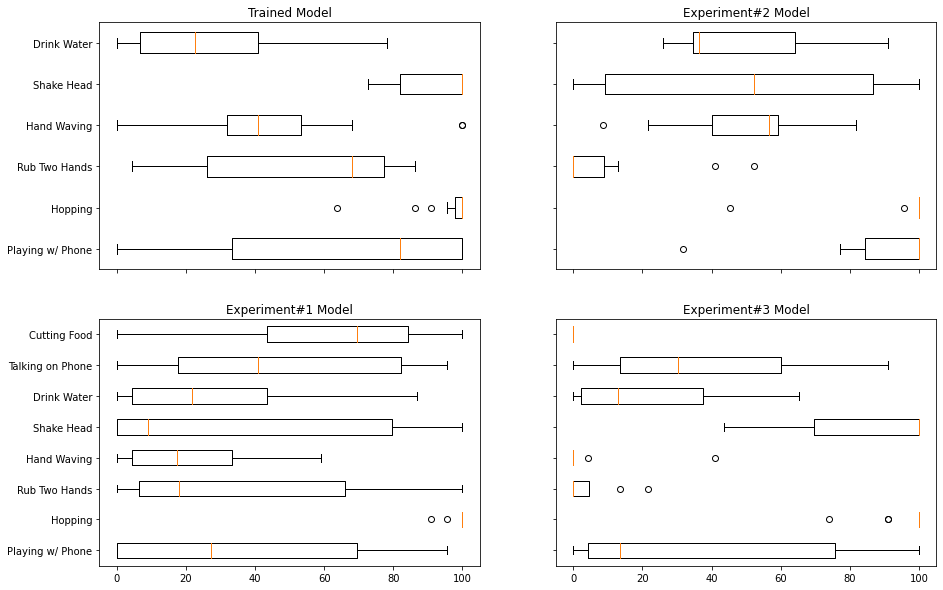
\includegraphics[width=\textwidth]{images/hri_boxplots.png}
            \caption{Per action results from HRI Study for each model}
      \end{figure} 
      \end{columns}
\end{frame}

\begin{frame}{HRI Study}
      \framesubtitle{Results}%
      
      \begin{figure}[ht!]
            \centering
            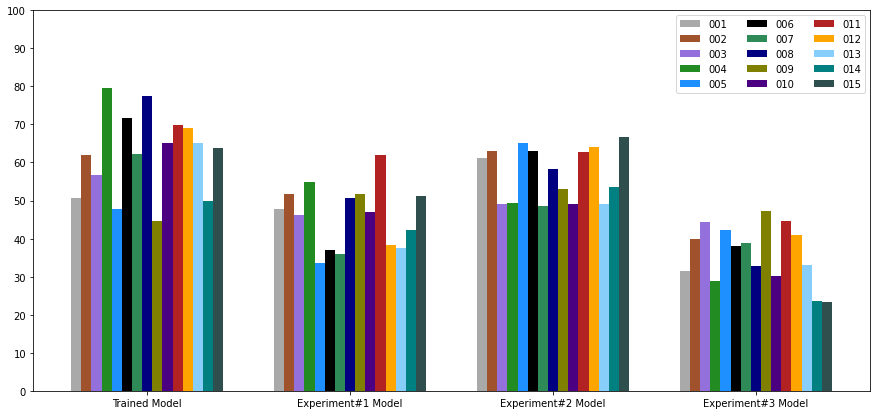
\includegraphics[width=0.8\textwidth]{images/hri_barplots.png}
            \caption{Per person results from HRI Study for each model}
      \end{figure} 
\end{frame}

\begin{frame}
      \framesubtitle{}%
      
      \vspace{1.25cm}
      \centering
      \Huge
      \emph{Thank You!}\\
      \vspace{0.25cm}
      \large
      Questions?
\end{frame}

\appendix

\begin{frame}
      \framesubtitle{}%
      
      \vspace{1.25cm}
      \centering
      \Huge
      \emph{Appendix}\\
\end{frame}

\begin{frame}{CTR-GCN Confusion Matrix}
      \framesubtitle{}%
      
      \begin{figure}[ht!]
            \centering
            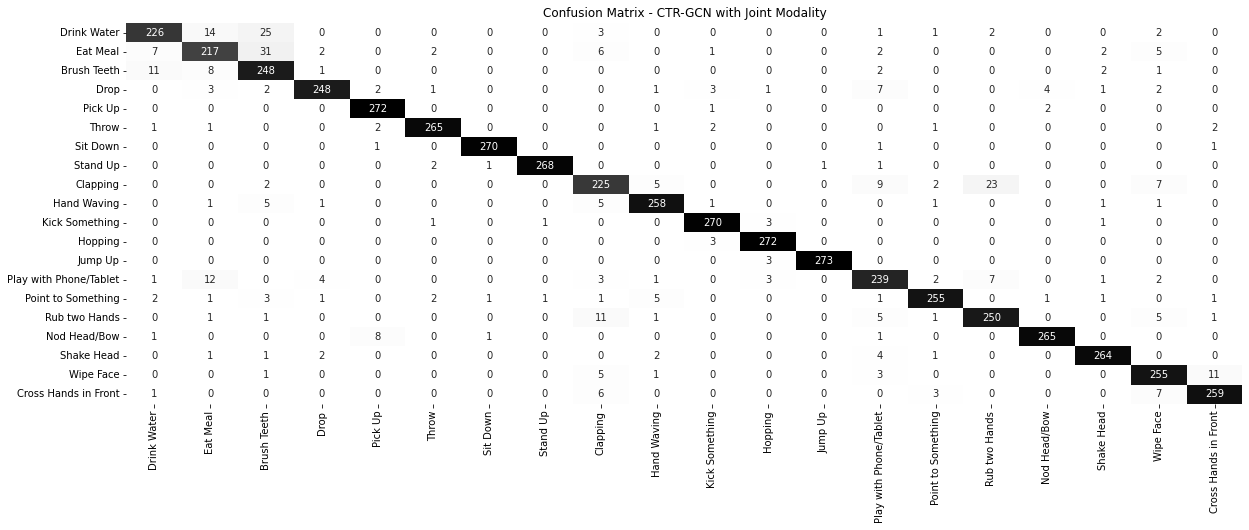
\includegraphics[width=\textwidth]{images/cf_ctr_jnt_cs.png}
            \caption{Cross-Subject confusion matrix of CTR-GCN network trained with joint data}
      \end{figure}
\end{frame}

\begin{frame}{CTR-GCN + BiC Confusion Matrix (NTU Joints)}
      \framesubtitle{}%
      
      \begin{figure}[ht!]
            \centering
            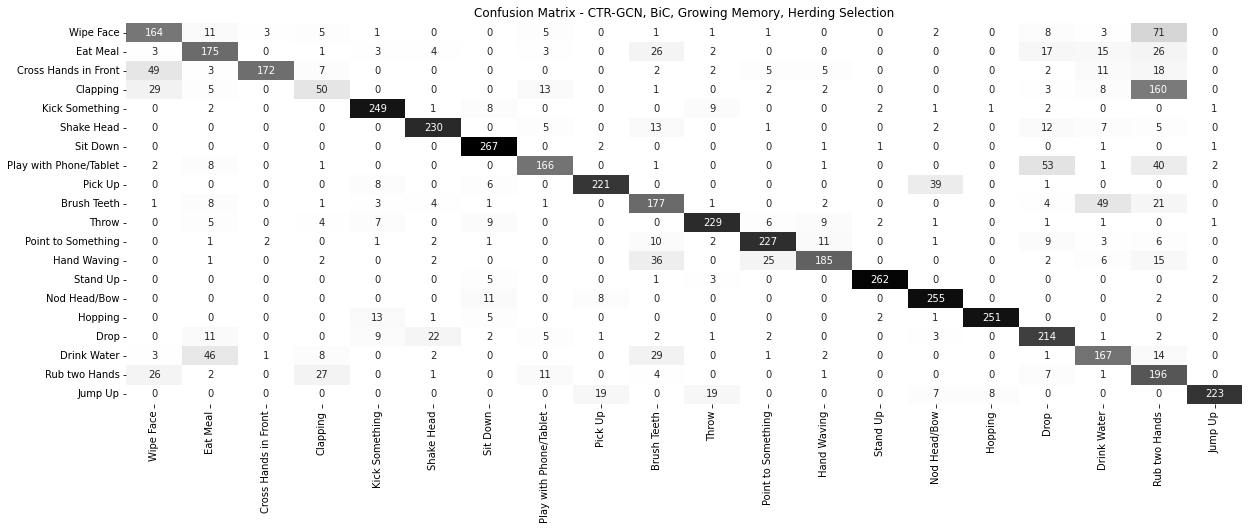
\includegraphics[width=\textwidth]{images/cf_ctr_bic_cs.png}
            \caption{Cross-Subject confusion matrix of CTR-GCN network and BiC IL approach}
      \end{figure}
\end{frame}

\begin{frame}{CTR-GCN + BiC Confusion Matrix (NT Joints)}
      \framesubtitle{}%
      
      \begin{figure}[ht!]
            \centering
            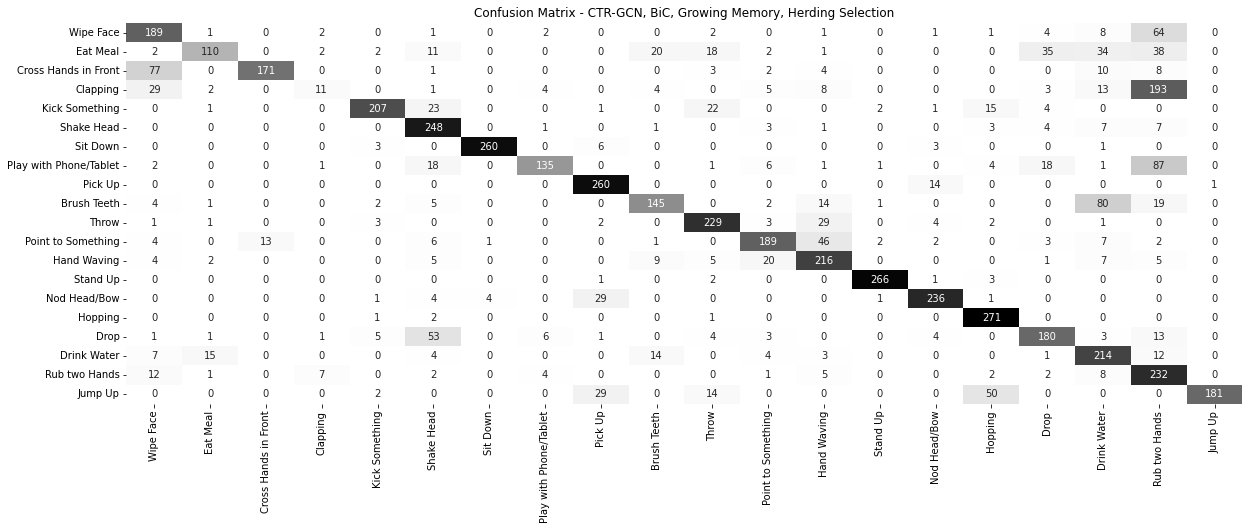
\includegraphics[width=\textwidth]{images/cf_ctr_bic_nt.png}
            \caption{Cross-Subject confusion matrix of CTR-GCN network and BiC IL approach}
      \end{figure}
\end{frame}

\begin{frame}{CTR-GCN, Fixed Results}
      \framesubtitle{}%
      
      \begin{columns}
      \column{0.5\textwidth}
      \begin{figure}[ht!]
            \centering
            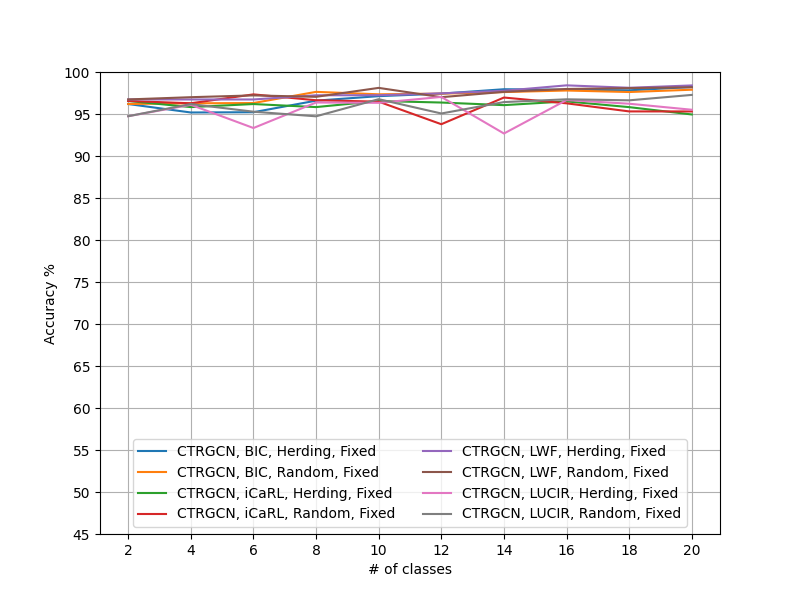
\includegraphics[width=\textwidth]{images/ctrgcn_fixed_TAw_Acc.png}
            \caption{Comparative task-aware accuracy w/ CTR-GCN  and fixed memory}
      \end{figure}
      
      \column{0.5\textwidth}
      \begin{figure}[ht!]
            \centering
            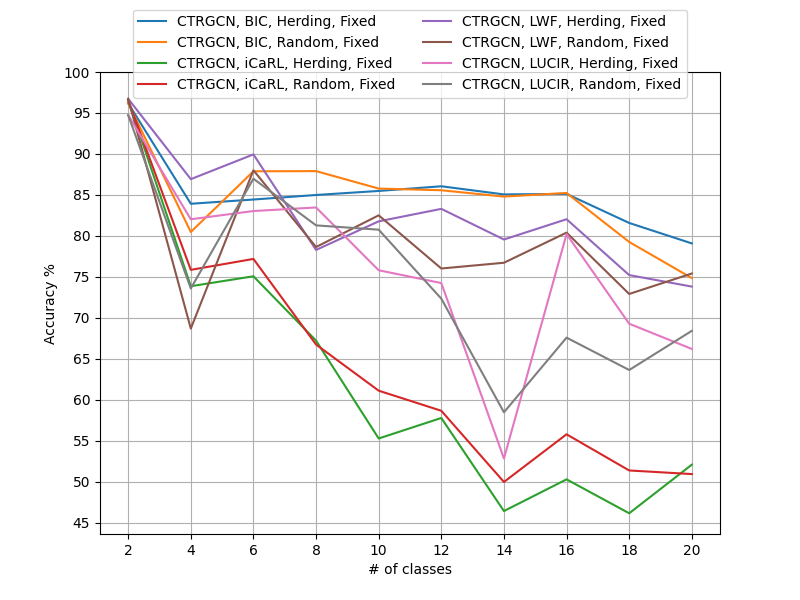
\includegraphics[width=\textwidth]{images/ctrgcn_fixed_TAg_Acc.png}
            \caption{Comparative task-agnostic accuracy w/ CTR-GCN  and fixed memory}
      \end{figure} 
      \end{columns}
\end{frame}

\begin{frame}{CTR-GCN, Growing Results}
      \framesubtitle{}%
      
      \begin{columns}
      \column{0.5\textwidth}
      \begin{figure}[ht!]
            \centering
            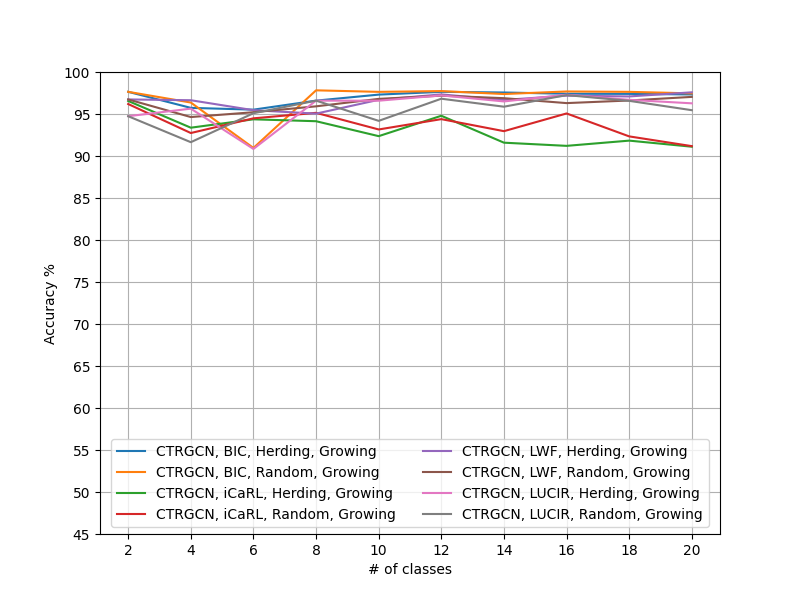
\includegraphics[width=\textwidth]{images/ctrgcn_growing_TAw_Acc.png}
            \caption{Comparative task-aware accuracy w/ CTR-GCN  and growing memory}
      \end{figure}
      
      \column{0.5\textwidth}
      \begin{figure}[ht!]
            \centering
            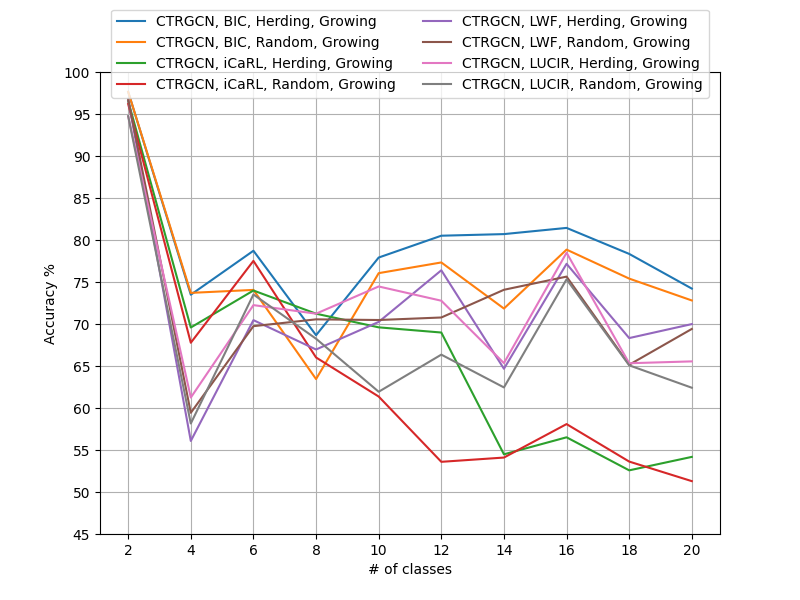
\includegraphics[width=\textwidth]{images/ctrgcn_growing_TAg_Acc.png}
            \caption{Comparative task-agnostic accuracy w/ CTR-GCN  and growing memory}
      \end{figure} 
      \end{columns}
\end{frame}

\begin{frame}{CTR-GCN + BiC (Per Task Accuracy)}
      \framesubtitle{}%
      
      \begin{figure}[ht!]
            \centering
            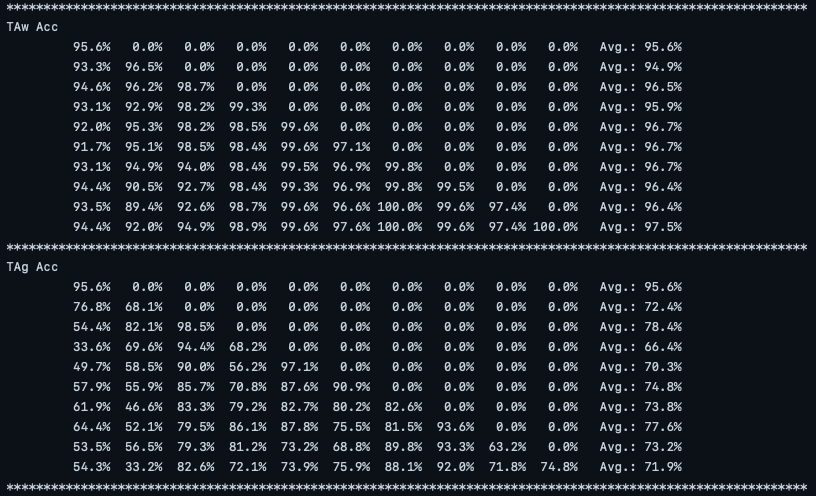
\includegraphics[width=0.7\textwidth]{images/per_task_acc}
            \caption{Task-aware and task-agnostic accuracy over task sequence}
      \end{figure}
\end{frame}

\begin{frame}{CTR-GCN + BiC (Per Task Forget)}
      \framesubtitle{}%
      
      \begin{figure}[ht!]
            \centering
            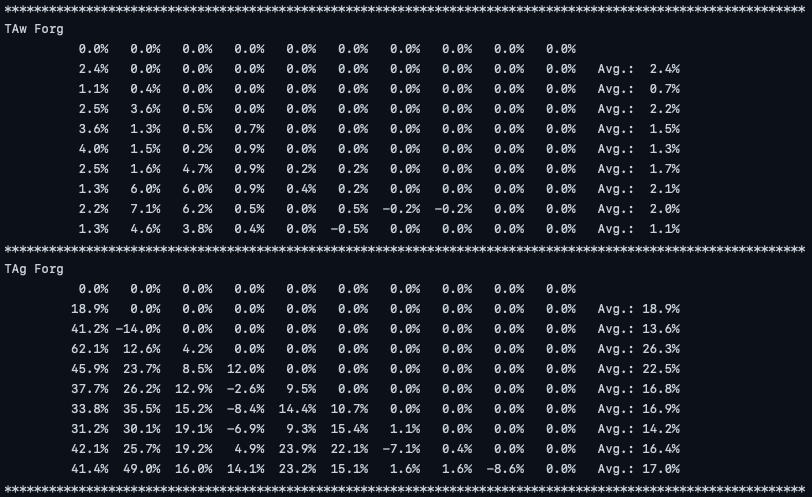
\includegraphics[width=0.7\textwidth]{images/per_task_forget}
            \caption{Task-aware and task-agnostic forgetting percentage over task sequence}
      \end{figure}
\end{frame}

\begin{frame}{Test Sequence \#1 Results}
      \framesubtitle{}%
      
      \begin{columns}
      \column{0.5\textwidth}
      \begin{figure}[ht!]
            \centering
            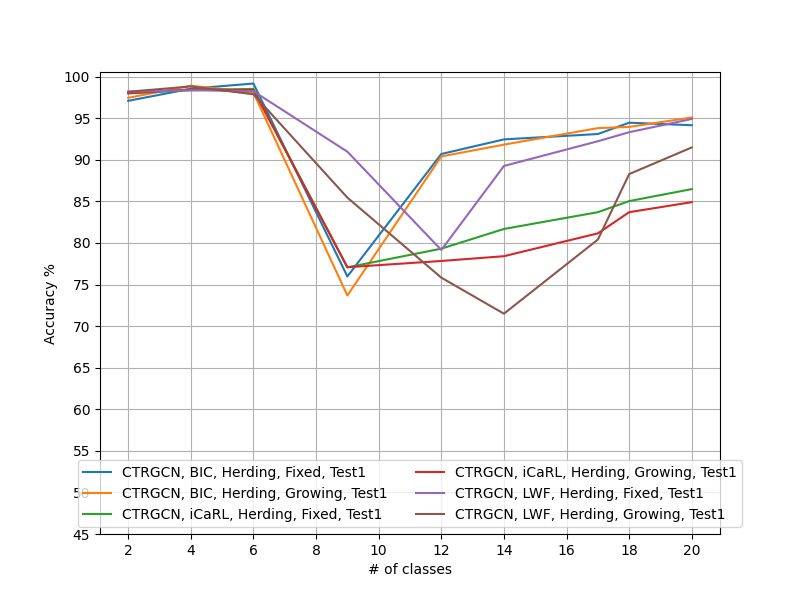
\includegraphics[width=\textwidth]{images/test_seq1_TAw_Acc.png}
            \caption{Task-agnostic accuracy for test sequence \#1}
      \end{figure}
      
      \column{0.5\textwidth}
      \begin{figure}[ht!]
            \centering
            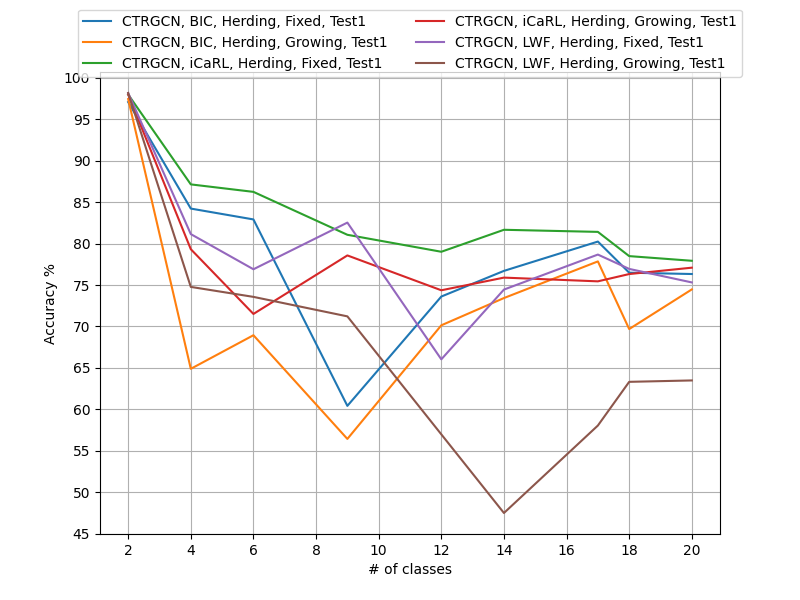
\includegraphics[width=\textwidth]{images/test_seq1_TAg_Acc.png}
            \caption{Task-aware accuracy for test sequence \#1}
      \end{figure} 
      \end{columns}
\end{frame}

\begin{frame}{Test Sequence \#2 Results}
      \framesubtitle{}%
      
      \begin{columns}
      \column{0.5\textwidth}
      \begin{figure}[ht!]
            \centering
            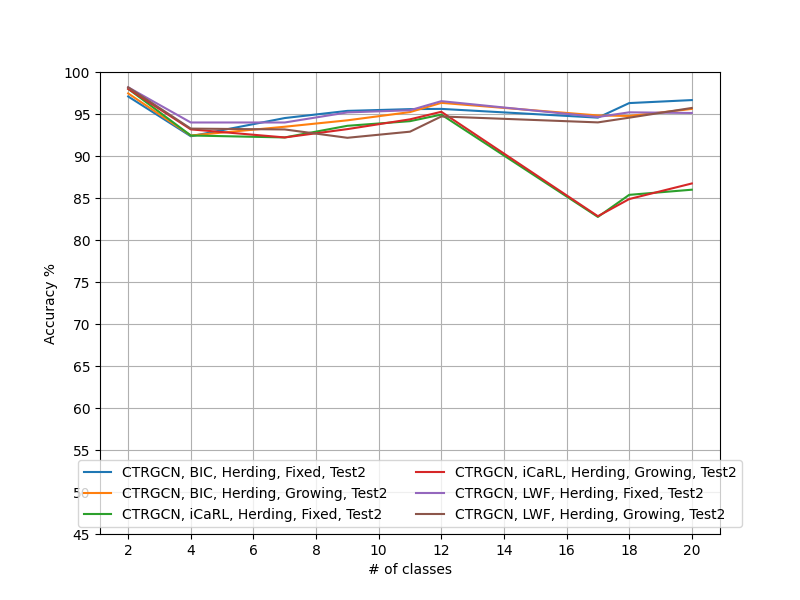
\includegraphics[width=\textwidth]{images/test_seq2_TAw_Acc.png}
            \caption{Task-aware accuracy for test sequence \#2}
      \end{figure}
      
      \column{0.5\textwidth}
      \begin{figure}[ht!]
            \centering
            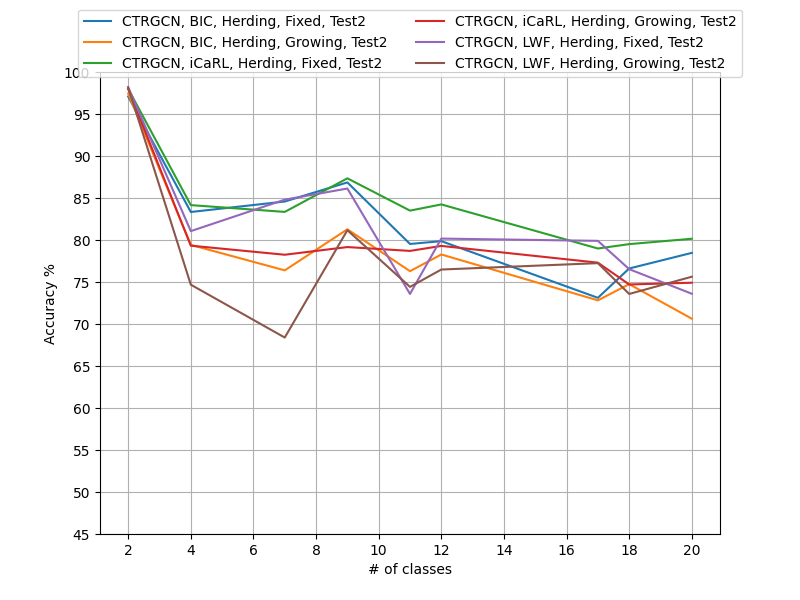
\includegraphics[width=\textwidth]{images/test_seq2_TAg_Acc.png}
            \caption{Task-agnostic accuracy for test sequence \#2}
      \end{figure} 
      \end{columns}
\end{frame}

\begin{frame}{Variable Memory Size Results}
      \framesubtitle{}%
      
      \begin{columns}
      \column{0.5\textwidth}
      \begin{figure}[ht!]
            \centering
            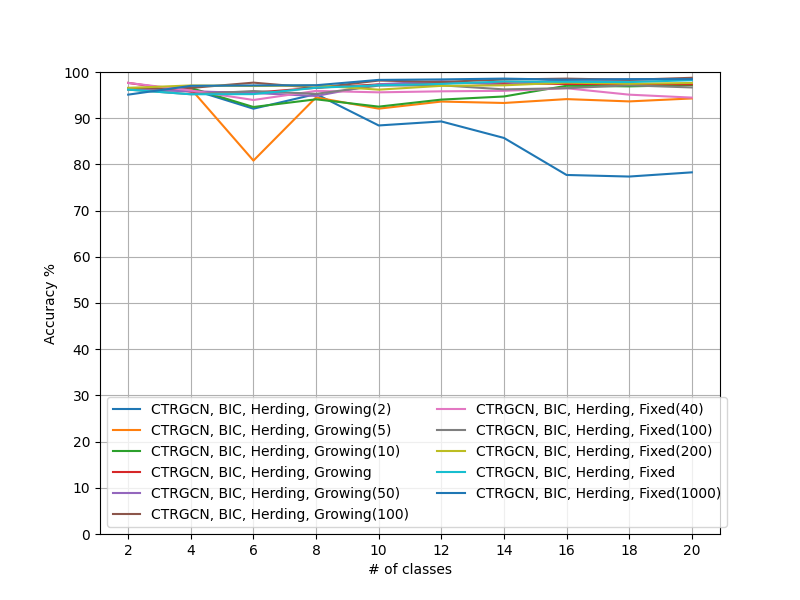
\includegraphics[width=\textwidth]{images/mem_sizes_TAw_Acc.png}
            \caption{Task-aware accuracy for varying memory size}
      \end{figure}
      
      \column{0.5\textwidth}
      \begin{figure}[ht!]
            \centering
            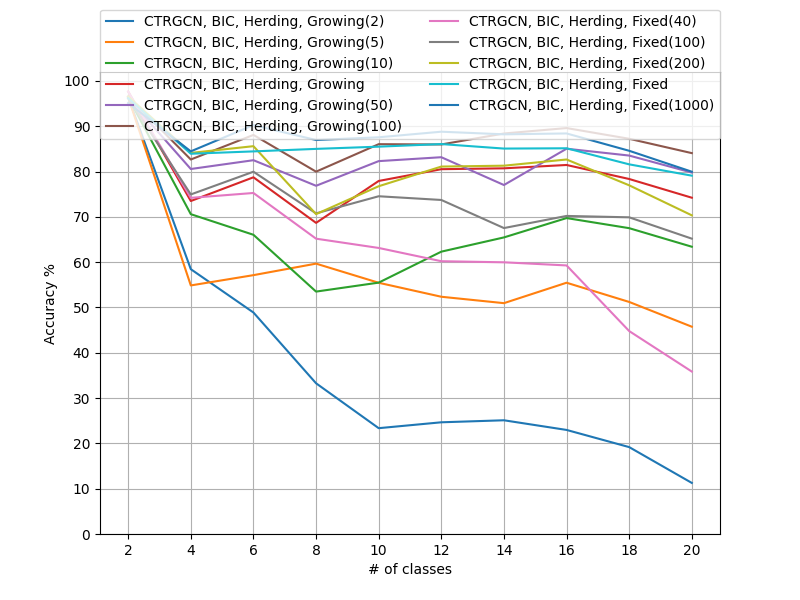
\includegraphics[width=\textwidth]{images/mem_sizes_TAg_Acc.png}
            \caption{Task-agnostic accuracy for varying memory size}
      \end{figure} 
      \end{columns}
\end{frame}

\begin{frame}{Incremental Learning Training}
      \framesubtitle{}%
      
      \vspace{-0.5cm}
      \begin{algorithm}[H]
      \begin{algorithmic}[1]
      \ENSURE $X^m, \ldots, X^n$ \hspace{0.25cm} // Training data 
      \ENSURE $K$ \hspace{0.25cm} // memory size
      \REQUIRE $\Theta$ \hspace{0.25cm} // current model
      \REQUIRE $P = (P_1, \ldots, P_{m-1})$ \hspace{0.25cm} // Exemplar set
      
      \STATE $\Theta \gets UpdateModel(X^n, \ldots, X^m, P, \Theta)$ \hspace{0.25cm} // Train model with new data
      \STATE $k \gets K/t$ \hspace{0.25cm} // update number of exemplars per class
      \FOR {$y = 1, \ldots, m-1$}
      \STATE $P_y \gets ReduceExemplars(P_y, k)$ \hspace{0.25cm} // reduce class exemplars to comply with m
      \ENDFOR
      \FOR {$y = m, \ldots, n$}
      \STATE $P_y \gets SelectExemplars(P_y, k, \Theta)$ \hspace{0.25cm} // Select exemplars for new classes
      \ENDFOR
      \STATE $P \gets (P_1, \ldots, P_{n})$ \hspace{0.25cm} // Update exemplar set
      \end{algorithmic}
      \caption{Incremental Learning Training Loop}
      \label{alg:iltrain}
      \end{algorithm}
\end{frame}

\begin{frame}{LwF Approach}
      \framesubtitle{}%
      
      \begin{columns}
      \column{0.5\textwidth}
      \begin{figure}[ht!]
            \centering
            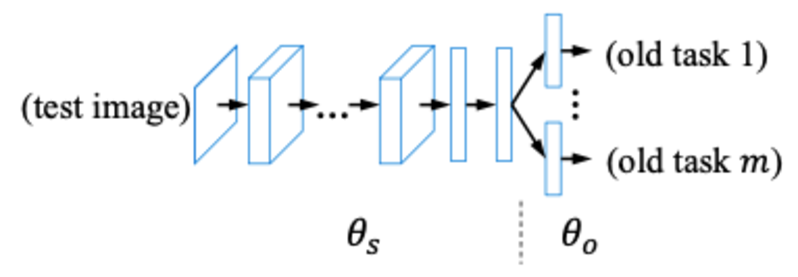
\includegraphics[width=0.6\textwidth]{images/lwf_cnn_model}
            \caption{Original CNN model\footnotemark[11]}
      \end{figure}
      
      \begin{figure}[ht!]
            \centering
            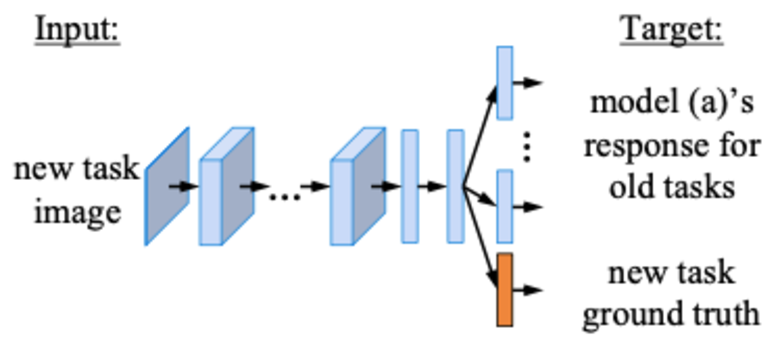
\includegraphics[width=0.6\textwidth]{images/lwf_model}
            \caption{LwF architecture\footnotemark[11]}
      \end{figure} 
      
      \column{0.5\textwidth}
      \begin{itemize}
      \item Total Loss\\
      \vspace{-0.25cm}
            {\small
            \begin{equation}
            %\centering
            L = \lambda_oL_{old} + L_{new}
            \end{equation}
            }
      \item Multinomial Logistic Loss\\
      \vspace{-0.25cm}
            {\small
            \begin{equation}
            %\centering
            L_{new} = -y_n * log\: \hat{y}_n
            \end{equation}
            }
      \item Knowledge Distillation Loss\\
      \vspace{-0.5cm}
            {\small
            \begin{equation}
            \begin{split}
            %\centering
            L_{old} = - \sum^{l}_{i=1} y^{'(l)}_o * log\: \hat{y}^{'(l)}_o
            \end{split}
            \end{equation}
            }
      \end{itemize}
      \end{columns}
      \footnotetext[11]{Z. Li and D. Hoiem, “Learning without Forgetting,” IEEE Trans. Pattern Analysis and Machine Intelligence, vol. 40, no. 12, pp. 2935–2947, Dec 2018.}
\end{frame}

\begin{frame}{iCaRL Approach}
      \framesubtitle{}%
      
      \begin{columns}
      \column{0.5\textwidth}
      \begin{figure}[ht!]
            \centering
            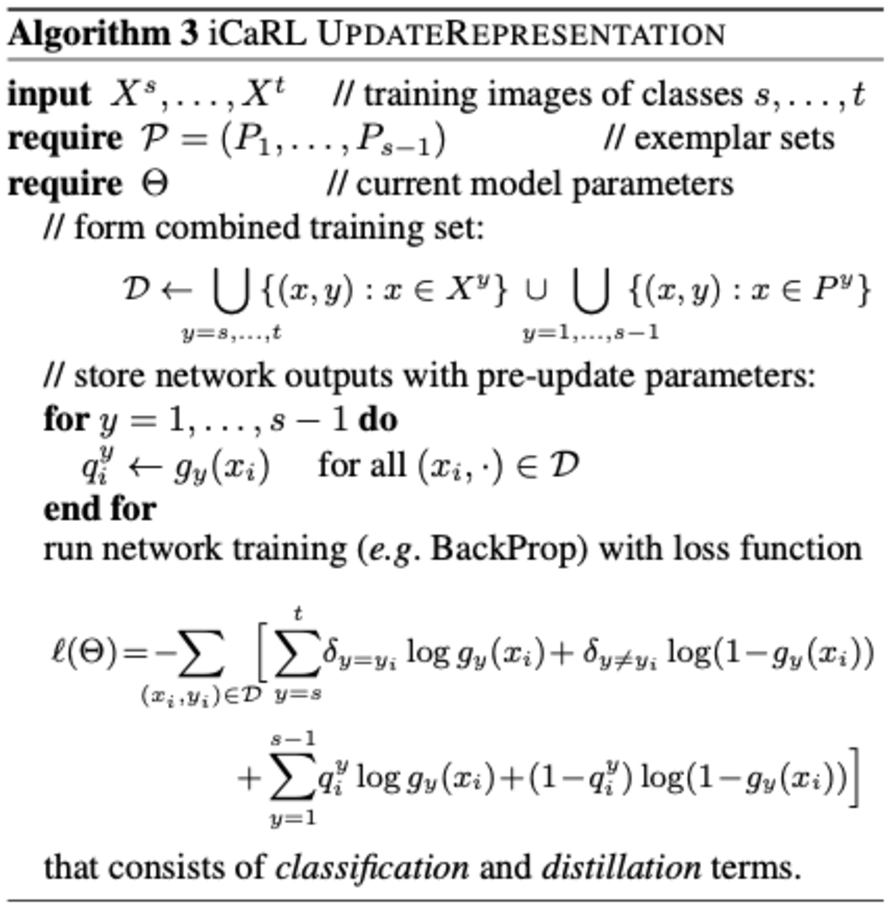
\includegraphics[width=0.7\textwidth]{images/icarl_algorithm3}
            \caption{iCaRL model training algorithm\footnotemark[12]}
      \end{figure}
      
      \column{0.5\textwidth}
      \begin{figure}[ht!]
            \centering
            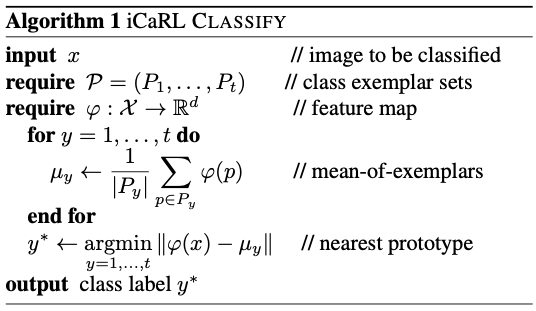
\includegraphics[width=0.8\textwidth]{images/icarl_algorithm1}
            \caption{iCaRL classifier algorithm\footnotemark[12]}
      \end{figure} 
      \end{columns}
      \footnotetext[12]{S.-A. Rebuffi, A. Kolesnikov, G. Sperl, and C. H. Lampert, “iCaRL: Incremental Classifier and Representation Learning,” in Proc. IEEE Conf. Computer Vision and Pattern Recognition (CVPR), 2017, pp. 5533–5542.}
\end{frame}

\begin{frame}{LUCIR Approach}
      \framesubtitle{}%
      
      \vspace{-0.5cm}
      \begin{columns}
      \column{0.5\textwidth}
      \vspace{-0.5cm}
      \begin{figure}[ht!]
            \centering
            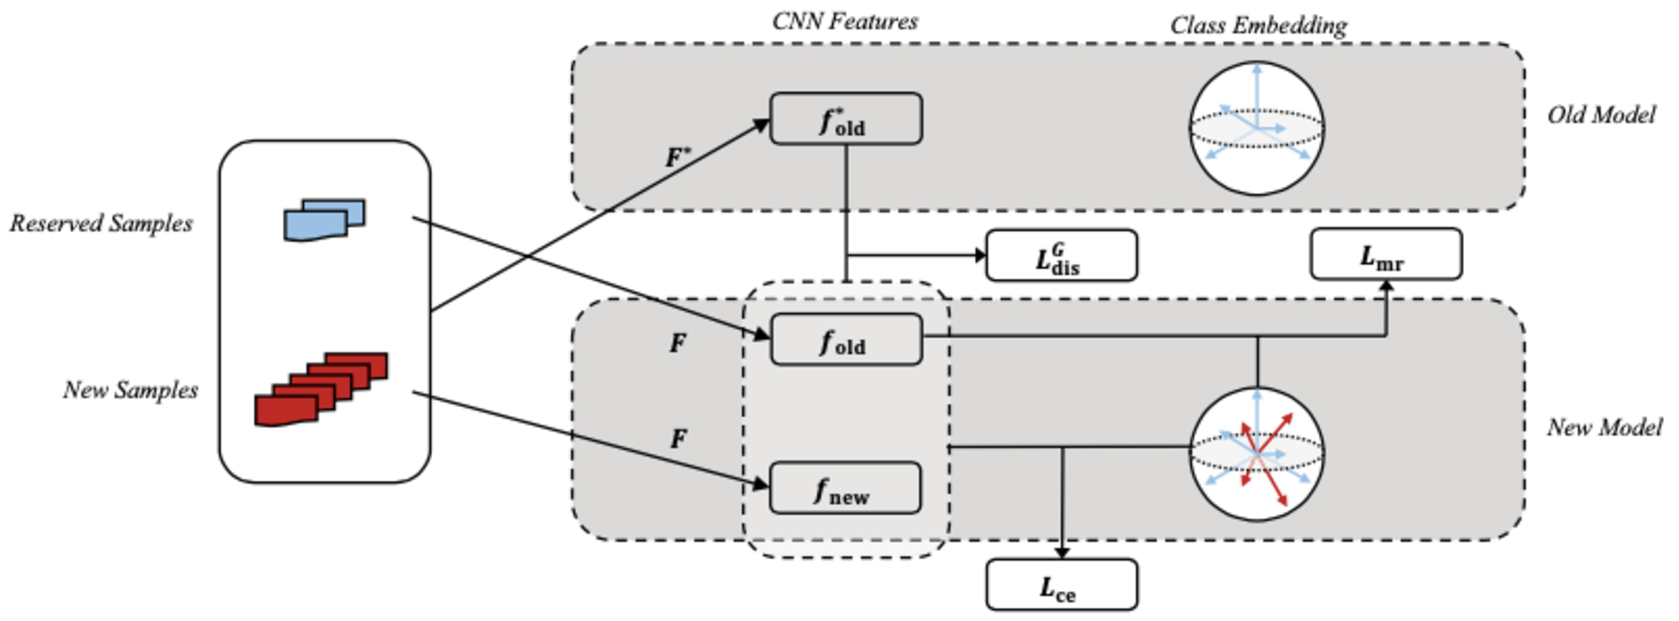
\includegraphics[width=1.05\textwidth]{images/lucir_approach.pdf}
            \caption{LUCIR approach\footnotemark[13]}
      \end{figure}
      
      \column{0.6\textwidth}
      \vspace{-0.5cm}
      \begin{itemize}
            \item Classification Loss\\
            \vspace{-0.5cm}
            {\small
            \begin{equation}
            %\centering
            L_{ce}(x) = - \sum^{|C|}_{i=1} y_i log (p_i)
            \end{equation}
            }
            \item Distillation Loss\\
            \vspace{-0.25cm}
            {\small
            \begin{equation}
            %\centering
            L^G_{dis}(x) = 1 - \langle \bar{f}^*(x), \bar{f}(x) \rangle
            \end{equation}
            }
            \item Margin Ranking Loss\\
            \vspace{-0.5cm}
            {\small
            \begin{equation}
            %\centering
            L_{mr}(x) = \sum^{K}_{k=1} max(m - \langle \bar{\theta}(x), \bar{f}(x) \rangle + \langle \bar{\theta}^k, \bar{f}(x) \rangle, 0)
            \end{equation}
            }
      \end{itemize}
      \end{columns}
      \begin{itemize}
      \item Total Loss\\
      \vspace{-0.5cm}
            {\small
            \begin{equation}
            %\centering
            L = \frac{1}{|N|} \sum_{x\in{N}} {(L_{ce}(x) + \lambda L^G_{dis}(x))} + \frac{1}{|N_o|} \sum_{x\in{N_o}} {L_{mr}(x)}
            \end{equation}
            }
      \end{itemize}
      \footnotetext[13]{S. Hou, X. Pan, C. C. Loy, Z. Wang, and D. Lin, “Learning a Unified Classifier Incrementally via Rebalancing,” in Proc. IEEE/CVF Conf. Computer Vision and Pattern Recognition (CVPR), 2019, pp. 831–839.}
\end{frame}

\begin{frame}{BiC Approach}
      \framesubtitle{}%
      
      \vspace{-0.75cm}
      \begin{columns}
      \column{0.525\textwidth}
      \begin{itemize}
      \item Total Loss\\
      \vspace{-0.5cm}
            {\small
            \begin{equation}
            %\centering
            L = \lambda L_d + (1 - \lambda) L_c
            \end{equation}
            }
      \item Classification Loss\\
      \vspace{-0.5cm}
            {\small
            \begin{equation}
            %\centering
            L_{ce}(x) = - \sum^{|C|}_{i=1} y_i log (p_i)
            \end{equation}
            }
      \item Distillation Loss\\
      \vspace{-0.75cm}
            {\small
            \begin{equation}
            \begin{split}
            %\centering
            L_d = \sum_{x\in{\hat{X}^n} \cup X^m} \sum^n_{k=1} -\hat{\pi}_k (x) log[\pi_k (x)],\\
            \hat{\pi}_k (x) = \frac{e^{\hat{o}_k (x)/T}}{\sum^n_{j=1}e^{\hat{o}_j (x)/T}}, \; \pi_k (x) = \frac{e^{o_k (x)/T}}{\sum^n_{j=1}e^{o_j (x)/T}}
            \end{split}
            \end{equation}
            }
      \end{itemize}
      
      \column{0.5\textwidth}
      \begin{figure}[ht!]
            \centering
            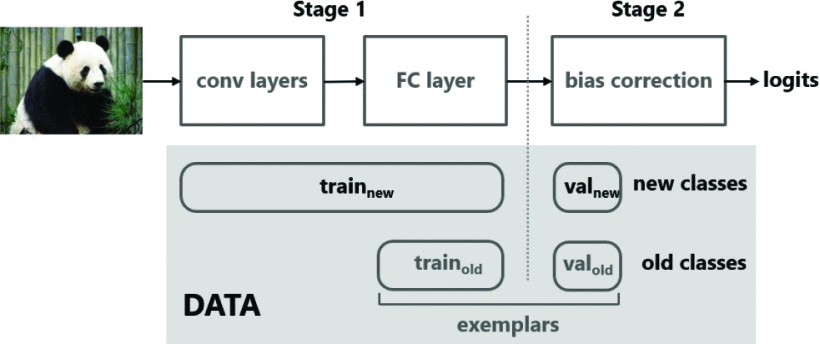
\includegraphics[width=0.9\textwidth]{images/bic_method}
            \caption{BiC approach\footnotemark[14]}
      \end{figure}
      \vspace{-0.5cm}
      \begin{itemize}
      \item Bias Correction Loss\\
      \vspace{-0.5cm}
            {\small
            \begin{equation}
            \begin{split}
            %\centering
            L_b = - \sum^{n+m}_{k=1} \delta_{y=k} log[softmax(q_k)],\\
            q_k =
            \begin{cases} 
            o_k & 1 \leq k \leq n \\
            \alpha o_k + \beta & n+1 \leq k \leq n+m 
            \end{cases}
            \end{split}
            \end{equation}
            }
      \end{itemize}
      \end{columns}
      \footnotetext[14]{Y. Wu et al., “Large Scale Incremental Learning,” in Proc. IEEE/CVF Conf. Computer Vision and Pattern Recognition (CVPR), 2019, pp. 374–382.}
\end{frame}

\begin{frame}{CTR-GCN Network}
      \framesubtitle{}%
      
      \vspace{-0.5cm}
      \begin{columns}
      \column{0.5\textwidth}
      \begin{figure}[ht!]
            \centering
            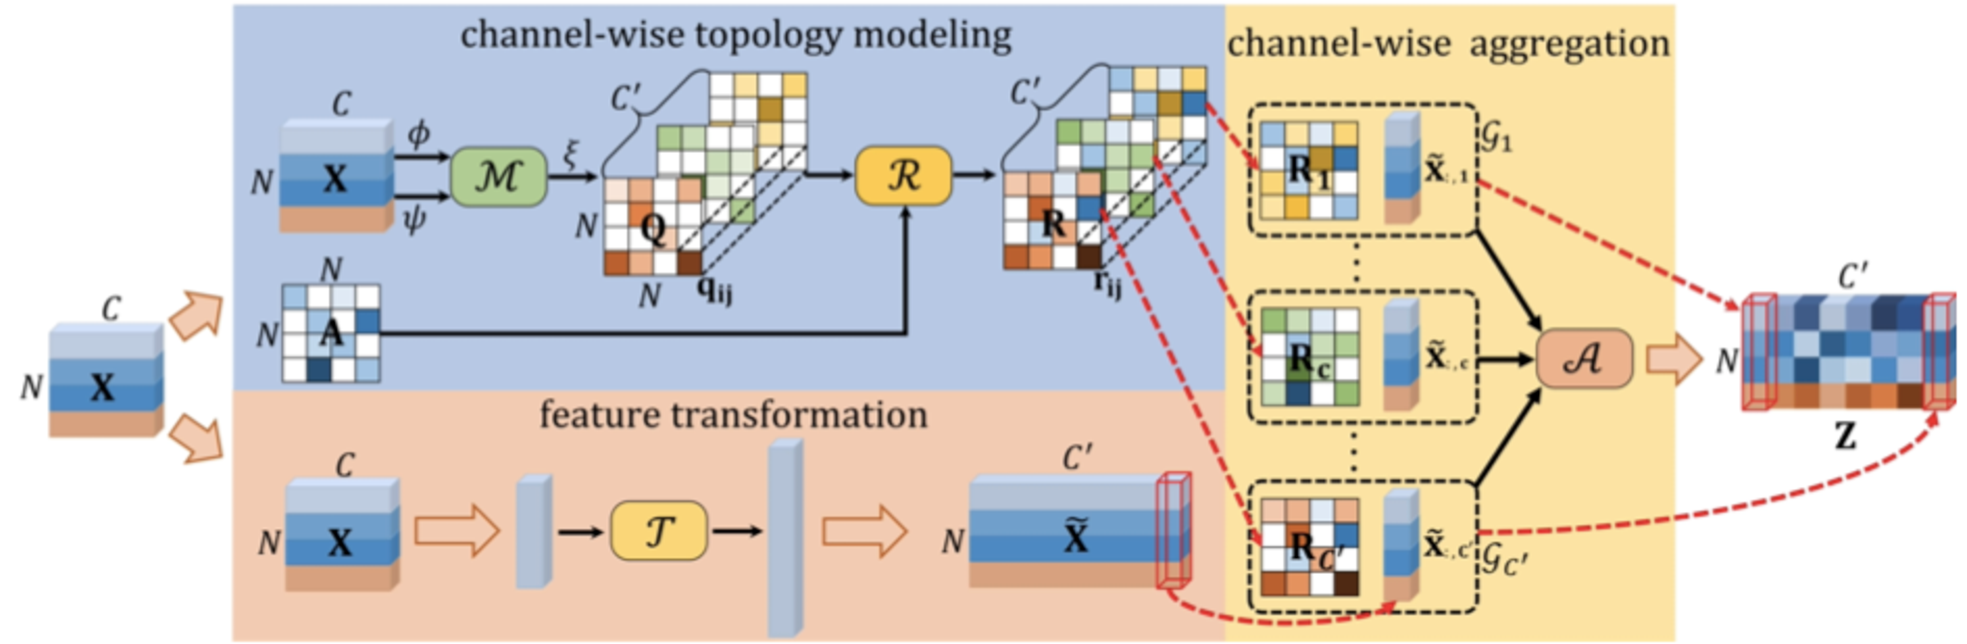
\includegraphics[width=\textwidth]{images/CTR-GC}
            \caption{CTR-GC block architecture\footnotemark[15]}
      \end{figure}
      
      \column{0.5\textwidth}
      \begin{figure}[ht!]
            \centering
            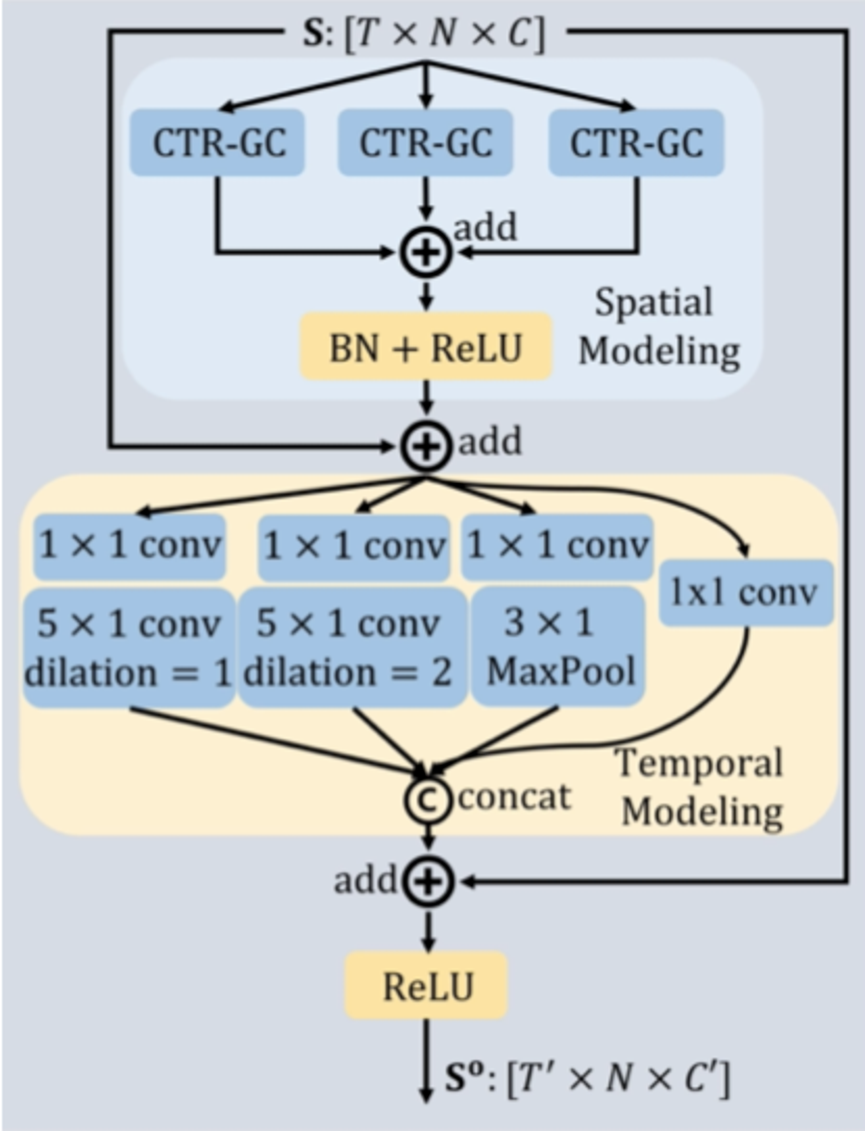
\includegraphics[width=0.6\textwidth]{images/CTR-GCN}
            \caption{CTR-GCN network architecture\footnotemark[15]}
      \end{figure} 
      \end{columns}
      \footnotetext[15]{Y. Chen et al., “Channel-Wise Topology Refinement Graph Convolution for Skeleton-Based Action Recognition,” in Proc. IEEE/CVF Int. Conf. Computer Vision (ICCV), 2021, pp. 13 359–13 368.}
\end{frame}

\begin{frame}{MS-G3D Network}
      \framesubtitle{}%
      
      \begin{figure}[ht!]
            \centering
            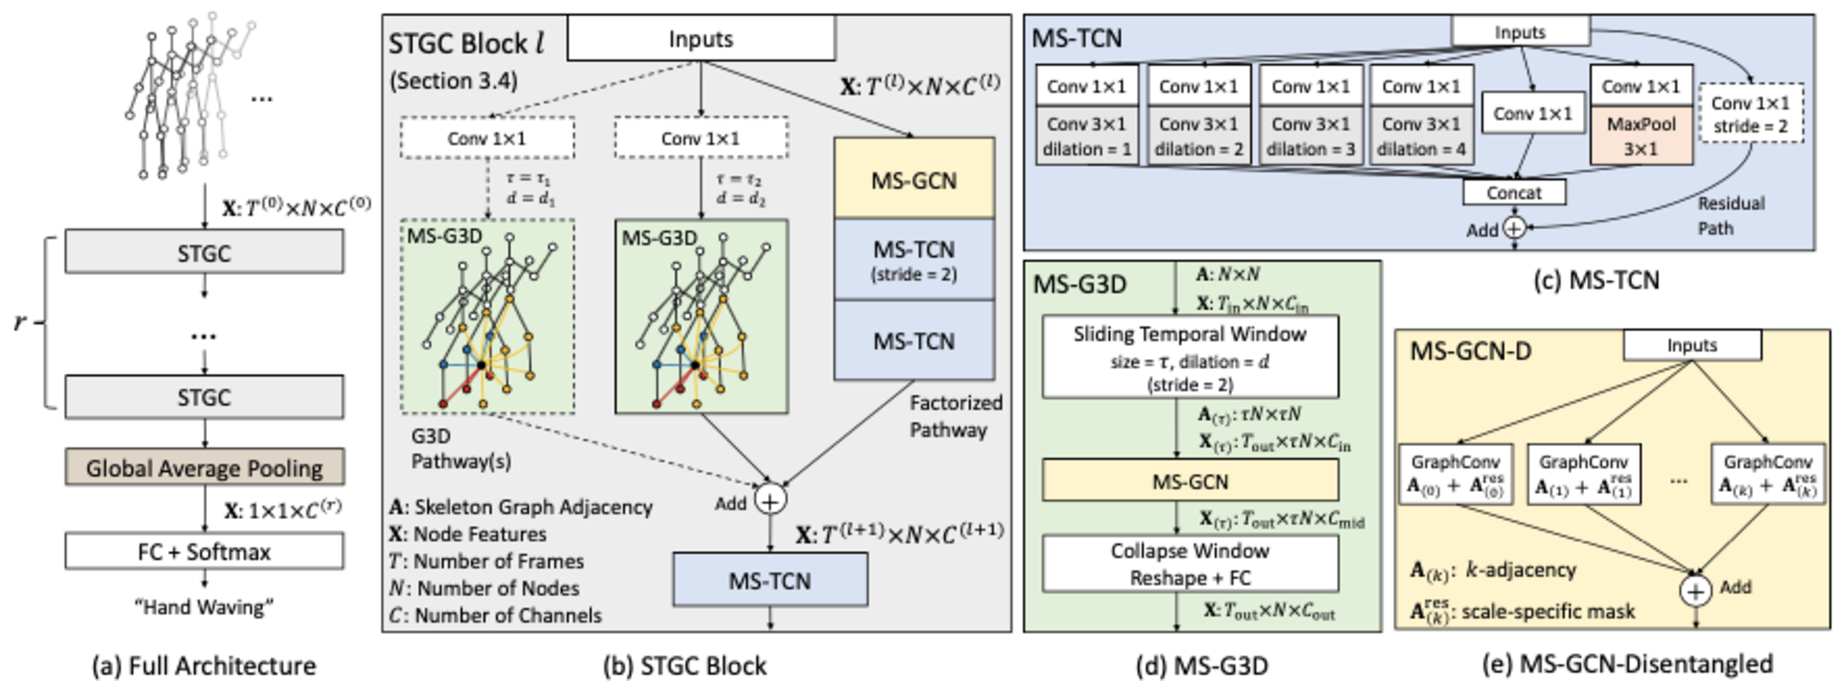
\includegraphics[width=\textwidth]{images/msg3d_arch}
            \caption{MS-G3D Architecture\footnotemark[16]}
            \footnotetext[16]{Z. Liu, H. Zhang, Z. Chen, Z. Wang, and W. Ouyang, “Disentangling and Unifying Graph Convolutions for Skeleton-Based Action Recognition,” in IEEE/CVF Conf. Computer Vision and Pattern Recognition (CVPR), 2020, pp. 140–149.}
      \end{figure}
\end{frame}

\end{document}
